\documentclass[12pt, eqno, limlimits]{article}
\usepackage[round, sort]{natbib}
\usepackage{amsfonts, amsmath, amssymb, amscd}
\usepackage{amsthm}
\usepackage[colorlinks=true,linkcolor=black,anchorcolor=black,citecolor=black,urlcolor=blue]{hyperref}
\usepackage{color, xcolor}
\usepackage{makecell}
\usepackage{latexsym}
\usepackage{algorithmicx}
\usepackage{enumerate}
\usepackage{tikz}
\usepackage{geometry}
\usepackage{multirow}
\usepackage{tabularx}
\usepackage{booktabs}
\usetikzlibrary{calc}
\usepackage{algorithm2e}
\usepackage{float}
\renewcommand{\floatpagefraction}{0.8}  
\renewcommand{\topfraction}{0.9}     
\renewcommand{\bottomfraction}{0.8}   
\textheight=24.5cm \textwidth=16.5cm
\parskip = 0.165cm
\renewcommand\baselinestretch{1.2}
\topmargin=-2cm \oddsidemargin=0cm \evensidemargin=0cm
\newtheorem{theorem}{Theorem}[section]
\newtheorem{cor}{Corollary}[section]
\newtheorem{lemma}{Lemma}[section]
\newtheorem{rem}{Remark}[section]
\newtheorem{definition}{Definition}[section]
\newtheorem{obs}{Observation}
\newtheorem{proposition}[theorem]{Proposition}
\newtheorem{exam}{Example}[section]
\title{\bf Maximizing the total weight of just-in-time jobs in a two-stage flexible flow shop with dedicated machines}
\author{Ren-Xia Chen$^{a}$, Shi-Sheng Li$^{a,}\footnote{Corresponding author.
        E-mail address: liss@zut.edu.cn (S.S. Li)}$, Xu-Hong Li$^{a}$, Jun-Ling Yuan$^{b}$\\
    {\small $^{a}$School of Mathematics and Information Science, Zhongyuan University of Technology,}\\
    {\small Zhengzhou 450007, People's Republic of China}\\
    {\small $^{b}$School of Electronics and Information, Zhengzhou University of Light Industry,}\\
    {\small Zhengzhou 450001, People's Republic of China}\\}
\date{}

\begin{document}
    \begin{sloppypar}
        \maketitle \hrule width\textwidth \ \\
        \textbf{Abstract:} We study a two-stage flexible flow shop scheduling problem aimed at maximizing the total weight of just-in-time jobs, defined as those that complete exactly on their due dates. Two machine configurations are examined: (i) a single common bottleneck machine at stage 1 and $m$ parallel dedicated machines at stage 2; (ii) $m$ parallel dedicated machines at stage 1 and a single common bottleneck machine at stage 2, where $m$ denotes the number of parallel dedicated machines. For the first configuration, we propose a pseudo-polynomial-time dynamic programming algorithm and a fully polynomial-time approximation scheme when $m$ is fixed. For the second configuration, we  establish that the problem is strongly $\mathcal{NP}$-hard for arbitrary $m$, even when all jobs have unit weight, and show that it remains ordinarily $\mathcal{NP}$-hard for $m=2$ under the same condition. We then design a pseudo-polynomial-time algorithm for fixed $m$.
        
        \noindent \textbf{Keywords:} Scheduling; Flexible flow shop; Dedicated machines; Just-in-time jobs
        
        \section{Introduction}
        
        Advances in production optimization research have shown that just-in-time (JIT) operations are very important in modern manufacturing systems. This importance arises from JIT's ability to simultaneously reduce inventory costs and enhance demand adaptability. In order to ensure that manufactured orders are completed exactly on their specified due dates, a key aspect of a JIT environment is the synchronization of production timelines with customer requirements. In this context, the objective is to find a schedule that minimizes the total penalty costs associated with either early or tardy job completions. Two main approaches are adopted to describe these penalty costs. The first approach assumes that each job’s penalty cost is proportional to its duration of earliness or tardiness deviations (\citealp{RolimNagano2020CIE}), and the second approach incurs a fixed penalty cost if a job is not completed exactly on its due date (\citealp{LannMosheiov1996COR}). A job is classified as \textit{JIT} in a schedule if it is completed exactly on its due date. In the literature, the minimization of total (weighted) earliness and tardiness is commonly termed the \textit{earliness-tardiness scheduling} problem, while the maximization of the  total weight of JIT jobs is characterized as the \textit{JIT scheduling} problem.
        
        The study of the two-machine flow shop scheduling problem, initiated by the seminal work of \cite{Johnson1954NRL}, remains a central topic in operations research. This area still generates significant academic and industrial interest, as shown by ongoing theoretical advancements and recent studies such as \cite{DolguiKovalyovLin2022NRL}, \cite{Shabtay2023NRL}, \cite{LvWang2024CIE},  and \cite{Perez-GonzalezFraminan2024EJOR}. Among the various flow shop scheduling configurations, the two-stage flexible flow shop with parallel dedicated machines (FF2PDM) scheduling stands out a crucial model that effectively integrates hybrid resource allocation with practical manufacturing requirements. In a typical FF2PDM setting, the system consists of two sequential processing stages with distinct machine configurations (\citealp{HwangLin2018COR}). One of these stages serves as a single common bottleneck machine, while the other stage employs parallel dedicated machines tailored for specific jobs. This framework closely mirrors real-world production systems that require the synchronized use of both dedicated and shared resources. For instance, in electronics manufacturing, printed circuit boards undergo a standardized soldering process on high-speed shared equipment before progressing to dedicated stations for customized functional testing. Similarly, in the automobile manufacturing, panels for different car models are initially molded and polished on dedicated production lines, followed by a centralized painting facility that handles the finished panels. The integration of shared and dedicated resources can not only enhance production efficiency but also address the complex challenges of modern manufacturing, which renders the FF2PDM scheduling an important research topic in current operations research. 
        
        The FF2PDM scheduling was originally pioneered by \cite{HerrmannLee1992} within the framework of look-ahead scheduling. They demonstrated that the problem of minimizing the maximum completion time is strongly $\mathcal{NP}$-hard, even when there is a common bottleneck machine at stage 1 and two parallel dedicated machines at stage 2. They also presented a $(2-\frac{1}{m})$-approximation algorithm for the general case with $m$ parallel dedicated machines at stage 2. \cite{HwangLin2018COR} explored FF2PDM scheduling models by optimizing two contrasting configurations: model 1 features a common bottleneck machine at stage 1 and $m$ parallel dedicated machines at stage 2 (denoted as $FF2(1, m)$), while model 2 reverses this setup with $m$ dedicated machines at stage 1 and a common bottleneck machine at stage 2 (denoted as $FF2(m, 1)$). They provided a comprehensive review of established models and results based on performance metrics, and developed novel algorithmic approaches with improved computational complexity. Due to its broad applications in manufacturing, the FF2PDM model has inspired numerous variants and extensions, as evidenced in recent studies such as \cite{ZhengHeYang2023COR}, \cite{HajjiHamlaoui2024AIME}, \cite{AgnetisMosheiov2025OPTL}, and \cite{ZhaoChenAn2025CIE}. Although studies on FF2PDM scheduling has advanced significantly, most studies have focused on minimizing regular objective functions such as the makespan and total completion time, while giving little attention to JIT-related criteria. In modern manufacturing, it is crucial to find schedules that maximize the number of products completed exactly on their due dates, as early or tardy completions may lead to excessive holding costs or late penalties. To address this practical need, we investigate a scheduling problem within the FF2PDM framework, aiming to maximize the total weight of JIT jobs.
        
        The JIT scheduling was first introduced by \cite{LannMosheiov1996COR}, who developed an $O(n^2)$-time algorithm for the single-machine case. They extended their work to a more general scenario where penalty costs for jobs are asymmetric, i.e., different costs arise depending on whether jobs are completed early or tardy. Note that when penalty costs are symmetric, maximizing the total weight of JIT jobs is equivalent to minimizing the total weight of early and tardy jobs.  \cite{HiraishiLevner2002COR} addressed JIT scheduling with positive set-up times on identical parallel machines. They established that this problem can be transformed into a 0-1 network transshipment problem. \cite{SungVlach2005JOS} explored JIT scheduling on $m$ unrelated parallel machines. They demonstrated that the problem is strongly $\mathcal{NP}$-hard for arbitrary $m$, and designed an $O(mn^{m+1})$-time algorithm for fixed $m$. \cite{JolaiAmalnick2011JIM} continued the work of \cite{SungVlach2005JOS} by proposing a hybrid memetic algorithm.
        
        \cite{ChoiYoon2007JOS} investigated JIT scheduling in a flow shop setting. They established that the two-machine weighted problem is binary $\mathcal{NP}$-hard and the three-machine unweighted problem is strongly $\mathcal{NP}$-hard. They also showed that the two-machine unweighted problem is solvable in $O(n^4)$ time. \cite{Shabtay2012EJOR} considered JIT scheduling in an $m$-machine flow-shop environment under three different variants. The first is a proportionate variant where job processing times are machine-independent, the second corresponds to identical jobs, and the third is a no-wait variant, where once a job is initiated on the first machine, it must process continuously through all $m$ machines without any interruption. \cite{ShabtayBensoussan2012JOS} demonstrated that the two-machine weighted problem is $\mathcal{NP}$-hard in the ordinary sense. To achieve this, they introduced a pseudo-polynomial-time dynamic programming (DP) algorithm and subsequently converted it into a fully polynomial-time approximation scheme (FPTAS), which runs in $O((n^4/\epsilon) \log(n/\epsilon))$ time. They also established that both the two-machine open shop and job shop problems are strongly $\mathcal{NP}$-hard. In addition, \cite{Elalouf2013JOS} provided an improved $O(n^3/\epsilon)$-time FPTAS for the two-machine weighted problem. Subsequent studies on JIT scheduling have investigated topics such as two-agent or multi-agent scheduling (\citealp{Yin2017JOS}; \citealp{Chen2019EngineeringOptimization}), scheduling with job rejection ( \citealp{MorMosheiov2022OperationalResearch}; \citealp{AtsmonyMosheiov2023JOS}), and distributed flow-shop scheduling (\citealp{Shabtay2023NRL}).
        
        Research on JIT scheduling is also closely related to the literature on machine scheduling with job rejection. In this setting, the scheduler must decide which jobs to accept for processing and which to reject by incurring a penalty (\citealp{ShabtayGasparKaspi2013JOS}). In JIT scheduling, jobs that cannot be completed exactly on their due dates are effectively rejected, as they contribute nothing to the objective value even if processed. Recent studies have examined rejection in single‑machine and parallel‑machine environments under various objective functions (e.g., \citealp{AtsmonyMosheiov2023JOS}; \citealp{LuOuYuZhang2023NRL}; \citealp{SangYW2025NRL}) as well as in two‑machine flow‑shop and job‑shop settings (e.g., \citealp{KimLee2022COR}; \citealp{ChenLi2024OPT}; \citealp{ShabtayGerstl2024EJOR}). However, to our knowledge, FF2PDM scheduling with rejection has not yet been investigated.
        
        Recently, \cite{HeegerHISShabtay2026} studied a scheduling problem that seeks to maximize the total weight of JIT jobs in the $FF2(1,m)$ configuration. They showed that for arbitrary $m$, the unweighted variant is strongly $\mathcal{NP}$-hard by a reduction from the Hitting Set problem. They also proposed a pseudo-polynomial-time backward DP algorithm and an FPTAS for the weighted version with fixed $m$. Their analysis further considered two special cases: (i) when the maximum processing time of any second-stage operation is bounded by a constant, and (ii) when the number of pairwise conflicting jobs is small. Some of their results are related to ours for $FF2(1,m)$. In particular, while both studies establish pseudo-polynomial-time algorithms and FPTASs for fixed $m$, their approaches differ significantly. Our forward DP algorithm, though it does not match their time complexity, provides a more intuitive framework that may simplify implementation. For our FPTAS, the rounding step utilizes a tighter lower bound, yielding comparable time complexity. This lower bound further enables a $2m$-approximation algorithm for the original problem. A key distinction is that \cite{HeegerHISShabtay2026} exclusively addressed $FF2(1,m)$, while our work covers both configurations comprehensively. We analyze $FF2(m,1)$ in depth, presenting two $\mathcal{NP}$-hardness results and a pseudo-polynomial-time algorithm, thus extending their $FF2(1,m)$ analysis.
        
        The structure of this paper is organized as follows. Section 2 provides the formal problem description. Section 3 presents our analysis of the $FF2(1,m)$ configuration: we first establish key properties of optimal schedules, then develop an exact DP algorithm, which is subsequently converted into an FPTAS for fixed $m$. In Section 4, we examine the $FF2(m,1)$ configuration, establishing strong $\mathcal{NP}$-hardness for arbitrary $m$ and ordinary $\mathcal{NP}$-hardness for $m=2$, followed by the development of a pseudo-polynomial-time algorithm for fixed $m$. Section 5 reports computational experiments on the algorithms proposed in Sections 3 and 4. Finally, Section 6 offers concluding remarks and research directions for future work.
        
        \section{Problem description}
        
        Consider a set $\mathcal{J}=\{J_1, J_2, \ldots, J_n\}$ of $n$ jobs. A subset of these jobs is to be scheduled as JIT jobs in an FF2PDM environment, while the remaining jobs are to be rejected. The $n$ jobs are categorized into $m$ disjoint groups $\mathcal{G}_1, \mathcal{G}_2, \ldots, \mathcal{G}_m$. Let $n_k=|\mathcal{G}_k|$ denote the number of jobs in $\mathcal{G}_k$, where $\sum_{k=1}^m n_k=n$. Each job $J_j \in \mathcal{J}$ comprises exactly two operations that need to be processed sequentially on their respective machines at stages 1 and 2. The job is characterized by a quintuple $\Phi_j=(a_j, b_j, d_j, w_j, g_j)$, where $a_j$ is the processing time at stage 1, $b_j$ is the processing time at stage 2, $d_j$ is the due date, $w_j$ is the weight (profit) obtained if it completes exactly on its due date (i.e., as a JIT job), and $g_j \in \{1, 2, \ldots, m\}$ is the group index, meaning $J_j \in \mathcal{G}_{g_j}$. All jobs are available at time zero, with no preemption allowed. 
        We assume the parameters $a_j$, $b_j$, $d_j$, and $w_j$ are positive integers. Two machine configurations are considered.
        \begin{itemize}
            \item Configuration $FF2(1, m)$: a single common bottleneck machine $M_0$ at stage 1, and $m$ parallel dedicated machines $M_1, M_2, \ldots, M_m$ at stage 2. All jobs are first processed on $M_0$, and after completion, the jobs in group $\mathcal{G}_k$ ($k=1, 2, \ldots, m$) proceed to their dedicated machine $M_k$ for the second-stage processing.
            
            \item Configuration $FF2(m, 1)$: $m$ parallel dedicated machines $M_1, M_2, \ldots, M_m$ at stage 1, and a single common bottleneck machine $M_0$ at stage 2. The jobs in group $\mathcal{G}_k$ ($k=1, 2, \ldots, m$) are first processed on their dedicated machine $M_k$, and upon completion, they are directed to $M_0$ for processing at stage 2.	
        \end{itemize} 
        
        Let $\mathcal{X}$ and $\overline{\mathcal{X}}$ be a partition of $\mathcal{J}$, i.e., $\mathcal{X} \cup \overline{\mathcal{X}}=\mathcal{J}$ and $\mathcal{X} \cap \overline{\mathcal{X}}=\emptyset$. This partition is referred to as a \textit{feasible partition} (or a \textit{feasible schedule}) if, for each $J_j \in \mathcal{X}$, its two operations can be scheduled in series on the two stage machines, with the second operation completing exactly on its due date. In a feasible schedule,  jobs in $\overline{\mathcal{X}}$ are assumed to be rejected and thus require no processing. The scheduling of the jobs in $\mathcal{X}$ is crucial and involves three key features: (i) the sequencing of jobs within each group $\mathcal{G}_k$ ($k=1, 2, \ldots, m$) on their dedicated machine $M_k$, (ii) the interleaving of the job sequences of the $m$ groups on the common bottleneck machine $M_0$, and (iii) the start times of two operations associated with each job in $\mathcal{X}$. In this context, $\mathcal{X}$ represents the set of JIT jobs and $\overline{\mathcal{X}}$ represents the set of rejected jobs in a feasible schedule. Our purpose is to identify a feasible schedule that maximizes the total weight of JIT jobs, i.e., to determine a feasible set $\mathcal{X}$ that maximizes $\sum_{J_j \in \mathcal{X}}w_j$. Following the traditional $\alpha \mid \beta \mid \gamma$ scheduling notation introduced by \cite{Graham1979AnDM} and extended to the FF2PDM framework by \cite{HwangLin2018COR}, the problems under study are denoted as $FF2(1, m)\mid \mid \sum_{J_j \in \mathcal{X}} w_j$ and $FF2(m, 1)\mid \mid \sum_{J_j \in \mathcal{X}} w_j$. When all jobs have unit weights (i.e., $w_j=1$ for $j=1, 2, \ldots, n$), the corresponding problems are written as $FF2(1, m)\mid \mid |\mathcal{X}|$ and $FF2(m, 1)\mid \mid |\mathcal{X}|$.
        
        Note that when there is only one dedicated machine (i.e., $m=1$), the $FF2(1, 1) \mid \mid \sum_{J_j \in \mathcal{X}} w_j$ problem reduces to the classical $F2 \mid \mid \sum_{J_j \in \mathcal{X}} w_j$ problem, which is $\mathcal{NP}$-hard in the ordinary sense (\citealp{ChoiYoon2007JOS}; \citealp{ShabtayBensoussan2012JOS}). This implies that both problems $FF2(1, m)\mid \mid \sum_{J_j \in \mathcal{X}} w_j$ and $FF2(m, 1)\mid \mid \sum_{J_j \in \mathcal{X}} w_j$ are at least binary $\mathcal{NP}$-hard for fixed $m$. 
        
        \begin{exam} \label{EX-2.1}
            Consider a 6-job instance of the $FF2(1, 2)\mid \mid \sum_{J_j \in \mathcal{X}} w_j$ problem, with job parameters listed in  Table \ref{TA-2.1}.
        \end{exam}
        
        \begin{table}[htpb]
            \footnotesize
            \caption{Job parameters for Example \ref{EX-2.1}} \label{TA-2.1} 
            \begin{center}
                \begin{tabular}{c|cccccc} 
                    $J_j$   & $J_1$ & $J_2$ & $J_3$ & $J_4$  & $J_5$ & $J_6$ \\ \hline
                    $a_j$   & 2 & 1  & 3 & 4 & 5 & 3   \\ 
                    $b_j$   & 3 & 4  & 2 & 4 & 4 & 6 \\ 
                    $d_j$   & 6 & 8  & 7 & 11 & 12 & 16 \\ 
                    $w_j$   & 3 & 2  & 3 & 4 & 7 & 5 \\ 
                    $g_j$   & 1 & 2  & 1 & 1 & 2 & 2 \\ \hline
                \end{tabular}
            \end{center}
        \end{table}
        
        For illustration, let the JIT set be $\mathcal{X} = \{J_1, J_2, J_5\}$, which has a total weight of 12. A feasible schedule for this set is depicted in Figure 1. This confirms feasibility, but this schedule is not optimal.
        
        \begin{center}
            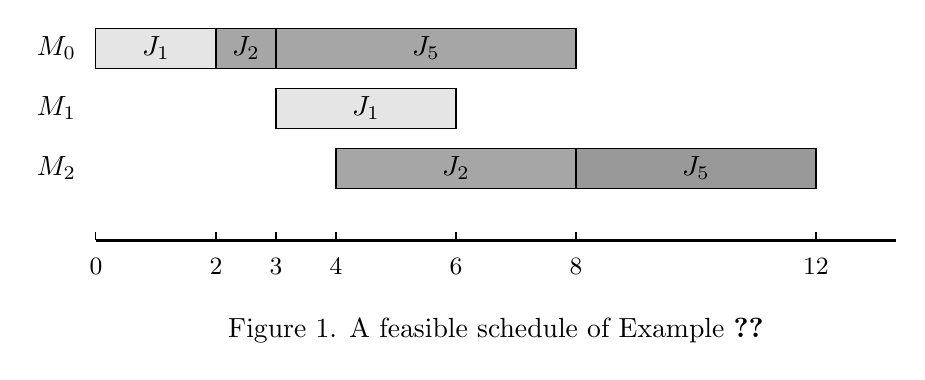
\begin{tikzpicture}[x=0.1in, y=0.2in]  \label{Figure-A.1}
                % machine index
                \node[anchor=east] at (-0.5,7) {$M_0$};
                \node[anchor=east] at (-0.5,5.5) {$M_1$};
                \node[anchor=east] at (-0.5,4) {$M_2$};
                
                % job on M_0
                \draw[fill=gray!20] (0,6.5) rectangle (6,7.5) node[midway] {$J_1$};
                \draw[fill=gray!70] (6,6.5) rectangle (9,7.5) node[midway] {$J_2$};
                \draw[fill=gray!70] (9,6.5) rectangle (24,7.5) node[midway] {$J_5$};
                
                % job on M_1
                \draw[fill=gray!20] (9,5) rectangle (18,6) node[midway] {$J_1$};
                
                % job on M_2
                \draw[fill=gray!70] (12,3.5) rectangle (24,4.5) node[midway] {$J_2$};
                \draw[fill=gray!80] (24,3.5) rectangle (36,4.5) node[midway] {$J_5$};
                
                % x-axis
                \draw[thick] (0,2.2) -- (40,2.2);
                \foreach \x/\label in {0/0, 6/2, 9/3, 12/4, 18/6, 24/8, 36/12} {
                    \draw (\x,2.2) -- (\x,2.4);
                    \node[below, font=\small] at (\x,2.0) {\label};
                }
                
                % caption
                \node[below] at (20,0.5) {Figure 1. A feasible schedule of Example \ref{EX-2.1}};
            \end{tikzpicture}
        \end{center}
        
        Without affecting generality, for both problems $FF2(1, m) \mid \mid \sum_{J_j \in \mathcal{X}} w_j$ and $FF2(m, 1) \mid \mid \sum_{J_j \in \mathcal{X}} w_j$, we assume $a_j+b_j \leq d_j$ for each $j=1, 2, \ldots, n$. If this condition does not hold, job $J_j$ can be deleted from the set $\mathcal{J}$, as it cannot be scheduled JIT in any feasible schedule. Moreover, let $J_0$ be a dummy job with $a_0=b_0=w_0=d_0=0$, and let $d_{\max}=\max\{d_j: j=1, 2, \ldots, n\}$ be the largest due date among all jobs in $\mathcal{J}$.
        
        \section{The $FF2(1, m)\mid \mid \sum_{J_j \in \mathcal{X}} w_j$ problem}
        
        In this section, we first establish several key structural properties of the $FF2(1, m)\mid \mid \sum_{J_j \in \mathcal{X}} w_j$ problem. Using these properties, we then develop an exact pseudo-polynomial-time DP algorithm for fixed $m$. Finally, we show how this algorithm can be transformed into an FPTAS.
        
        Given that the second operation of each JIT job must be processed within the time interval $[d_j-b_j, d_j]$ on 
        machine $M_{g_j}$, completing its first operation earlier on $M_0$ will not compromise this constraint. Hence, any idle time on $M_0$ can be eliminated by advancing subsequent jobs. This feature leads directly to the following result.
        
        \begin{lemma} \label{L-3.1}
            For the $FF2(1, m)\mid \mid \sum_{J_j \in \mathcal{X}} w_j$ problem, an optimal schedule exists such that the common bottleneck machine $M_0$ processes jobs continuously without idle times.
        \end{lemma}
        
        According to \cite{ChoiYoon2007JOS}, the $F2\mid \mid \sum_{J_j \in \mathcal{X}} w_j$ problem admits an optimal solution in which the JIT jobs are processed in the earliest due date (EDD) order on both machines. However, this property does not hold for the $FF2(1, m)\mid \mid \sum_{J_j \in \mathcal{X}} w_j$ problem even when $m=2$. Consider a 2-job instance of the $FF2(1, 2)\mid \mid \sum_{J_j \in \mathcal{X}} w_j$ problem, where $\Phi_1=(3, 2, 6, 4, 1)$ and $\Phi_2=(1, 8, 10, 5, 2)$. The optimal schedule has two JIT jobs, in which $J_2$ and $J_1$ are processed on $M_0$ during the intervals $[0,1]$ and $[1, 4]$, respectively, while $J_1$ is processed on $M_1$ during the interval $[4,6]$ and $J_2$ is processed  on $M_2$ during the interval $[2,10]$. However, if $J_1$ is processed before $J_2$ on $M_0$  (i.e., these two jobs are processed in EDD order), then the earliest completion time of $J_2$ is 12, which is larger than $10$.  Despite the invalidity of the EDD order for the $FF2(1, m)$ problem, we can still characterize a fundamental structural property of an optimal schedule, as formalized below. 
        
        \begin{lemma} \label{L-3.2}
            For the $FF2(1, m)\mid \mid \sum_{J_j \in \mathcal{X}} w_j$ problem, an optimal schedule exists such that: (i) on each dedicated machine $M_k$ ($k=1, 2, \ldots, m$), the JIT jobs in $\mathcal{X} \cap \mathcal{G}_k$ are processed in increasing order of $d_j-b_j$ ; and (ii) on the common bottleneck machine $M_0$, the JIT jobs in $\mathcal{X}$ are processed in non-decreasing order of $d_j-b_j$.
        \end{lemma}
        
        \noindent \textbf{Proof.} Owing to the facts that all JIT jobs must be completed exactly on their due dates and no two jobs can overlap on the same machine, the JIT jobs in group $\mathcal{G}_k$ ($k=1, 2, \ldots, m$) must be processed on $M_k$ in increasing order of $d_j-b_j$ (which is consistent with their EDD order) in any optimal schedule. This establishes property (i).
        
        Next, let $\sigma$ be an optimal schedule satisfying property (i) but violating property (ii).
        Then, two adjacent JIT jobs $J_u$ and $J_v$ on $M_0$ must satisfy $d_u-b_u > d_v-b_v$, where $J_u$ is sequenced just before $J_v$ in $\sigma$. An alternative schedule $\sigma'$ can be created from $\sigma$ by swapping positions of $J_u$ and $J_v$ on $M_0$. This swapping does not make $J_u$ and $J_v$ on their dedicated machine (or machines) shifted to the right. Apply this swapping procedure to $M_0$ a finite number of times, we obtain an optimal schedule satisfying both properties (i) and (ii). \hfill$\Box$\\
        
        Owing to Lemmas \ref{L-3.1} and \ref{L-3.2}, for the $FF2(1, m) \mid \mid \sum_{J_j \in \mathcal{X}} w_j$ problem, an optimal schedule can be fully determined by an optimal partition of $\mathcal{J}$ into a set $\mathcal{X}$ of JIT jobs and its complement $\overline{\mathcal{X}}=\mathcal{J} \setminus \mathcal{X}$ of rejected jobs. To simplify the presentation, the $n$ jobs are assumed to be numbered in non-decreasing order of $d_j-b_j$ throughout this section, i.e.,
        \begin{equation}\label{E-3.0}
            d_1-b_1 \leq d_2-b_2 \leq \cdots \leq d_n-b_n,
        \end{equation}
        where ties are broken arbitrarily.
        
        \subsection{A DP algorithm for the $FF2(1, m)\mid \mid \sum_{J_j \in \mathcal{X}} w_j$ problem}
        
        By utilizing the results of Lemmas \ref{L-3.1} and \ref{L-3.2}, we  propose an exact DP algorithm to solve the $FF2(1, m) \mid \mid \sum_{J_j \in \mathcal{X}} w_j$ problem. When $m$ is fixed, the algorithm runs in pseudo-polynomial time, demonstrating that the problem is $\mathcal{NP}$-hard in the ordinary sense.    
        
        For $j=1, 2, \ldots, n$, let $\mathcal{J}_j=\{J_1, J_2, \ldots, J_j\}$ denote the set of the first $j$ jobs in  $\mathcal{J}$. We outline a DP approach for the $FF2(1, m)\mid \mid \sum_{J_j \in \mathcal{X}} w_j$ problem. Consider a feasible partial schedule on $\mathcal{J}_j$ that satisfies Lemmas \ref{L-3.1} and \ref{L-3.2} and includes $J_j$ as a JIT job. Denote by $\mathcal{X}_j$ the set of JIT jobs in this schedule and by $\overline{\mathcal{X}}_j$ its complement. Every such feasible partial schedule can be uniquely represented by an $(m+3)$-dimensional tuple $(l_1, l_2, \ldots, l_m, T, W, \mathcal{X}_j)$, subject to the following conditions:
        \begin{description}
            \item (C1) For each $k=1, 2, \ldots, m$, $l_k=\arg_r \max\{J_r \in \mathcal{X}_j \cap \mathcal{G}_k\}$ denotes the maximal index in $\mathcal{X}_j \cap \mathcal{G}_k$ (if $\mathcal{X}_j \cap \mathcal{G}_k=\emptyset$, define $l_k=0$);
            
            \item (C2) $T=\sum_{J_i \in \mathcal{X}_j} a_i$ denotes the total processing time of JIT jobs in $\mathcal{X}_j$ on $M_0$;
            
            \item (C3) $W=\sum_{J_i \in \mathcal{X}_j} w_i$ denotes the total weight of JIT jobs in $\mathcal{X}_j$;
            
            \item (C4) $j=l_{g_j}=\max\{l_k: k=1, 2, \ldots, m\}$, i.e., $J_j \in \mathcal{X}_j$.
        \end{description}
        From these definitions, we have: (i) $\sum_{k=1}^m a_{l_k} \leq T \leq \sum_{i=1}^j a_i$, where $a_{l_k}=0$ if $l_k=0$; (ii) $\sum_{k=1}^m w_{l_k} \leq W \leq \sum_{i=1}^j w_i$, where $w_{l_k}=0$ if $l_k=0$; and (iii) $J_{l_k} \in \mathcal{G}_k$ if $l_k>0$. Note that (C1) means that the last JIT job on $M_k$ is $J_{l_k}$ if $l_k>0$; (C2) indicates that the completion time of the last JIT job's first operation on $M_0$ is exactly $T$; and (C4) implies that $J_j$ is a JIT job and, by Lemma \ref{L-3.2}, it should be scheduled last on $M_0$. The set $\mathcal{X}_j$ is recorded only for constructing the final optimal schedule.
        
        For each $j=1, 2,  \ldots, n$, let $\mathcal{D}_j$ be the set of all tuples corresponding to feasible partial schedules on $\mathcal{J}_j$ that satisfy conditions (C1)-(C4). To derive the tuple transition process, consider a tuple $(l'_1, l'_2, \ldots, l'_m, T', W', \mathcal{X}'_j) \in \mathcal{D}_j$ and let $\pi$ be a corresponding feasible partial schedule on $\mathcal{J}_j$. By definition, the set of JIT jobs in $\pi$ is $\mathcal{X}'_j$, $j=l'_{g_j}=\max\{l'_k: k=1, 2, \ldots, m\}$, $J_j$ is scheduled last on $M_0$, and its first operation's completion time is exactly $T'$. Because $J_j$ is a JIT job, its second operation must be processed on $M_{g_j}$  within the interval $[d_j-b_j, d_j]$. This implies two conditions: 
        \begin{description}
            \item (C5) The first operation of $J_j$ on $M_0$ finish by time $d_j-b_j$, so $T'\leq d_j-b_j$. 
            
            \item (C6) Any preceding JIT job (if any) on $M_{g_j}$ must finish by time $d_j-b_j$. 
        \end{description}
        Let $J_h$ be the second-to-last JIT job processed on $M_0$ in $\pi$. By Lemma \ref{L-3.2}, we have $h=\arg_k \max\{J_k \in \mathcal{X}'_j \setminus \{J_j\}\}$. Moreover, let $J_v$ be the second-to-last JIT job processed on $M_{g_j}$ in $\pi$. By Lemma \ref{L-3.2} and condition (C6), we have $v=\arg_k \max\{J_k \in (\mathcal{X}'_j \setminus \{J_j\}) \cap \mathcal{G}_{g_j}\}$ and  $d_v \leq d_j-b_j$. By removing $J_j$ from $\pi$, we obtain a partial schedule $\pi'$ on $\mathcal{J}_h$. This schedule is feasible for $\mathcal{J}_h$, satisfies Lemmas \ref{L-3.1} and \ref{L-3.2}, and has  $\mathcal{X}'_j \setminus \{J_j\}$ as its JIT job set. Consequently, $h=\max \{l'_1, l'_2, \ldots, l'_{g_j-1}, v, l'_{g_j+1}, \ldots, l'_m\}$ and the tuple corresponding to $\pi'$ is 
        $(l'_1, l'_2, \ldots, l'_{g_j-1}, v, l'_{g_j+1}, \ldots, l'_m, T'-a_j, W'-w_j, \mathcal{X}'_j \setminus \{J_j\})$. Clearly, this tuple belongs to $\mathcal{D}_h$. The above discussion shows that every tuple in $\mathcal{D}_j$ can be generated from a tuple in $\mathcal{D}_h$ for some $h \in \{0, 1,  \ldots, j-1\}$.
        
        The algorithm is initialized with $\mathcal{D}_0=\{(l_1=0, l_2=0, \ldots, l_m=0, T=0, W=0, \mathcal{X}_0=\emptyset)\}$, which corresponds to a dummy schedule. In the $j$-th iteration ($1 \leq j \leq n$), the tuple set $\mathcal{D}_j$ is constructed dynamically from the previous generated sets $\mathcal{D}_0, \mathcal{D}_{1}, \ldots, \mathcal{D}_{j-1}$. For each $h=0, 1, \ldots, j-1$, let $\mathcal{D}_{j,h} \subseteq \mathcal{D}_j$ denote the subset of tuples in which the second-to-last JIT job on $M_0$ is $J_h$. Then for any feasible partial schedule on $\mathcal{J}_j$ that corresponds to a tuple in $\mathcal{D}_{j,h}$, the jobs $J_{h+1}, J_{h+2}, \ldots, J_{j-1}$ are rejected. As a consequence, for each tuple $(l_1, l_2, \ldots, l_m, T, W, \mathcal{X}_h) \in \mathcal{D}_h$, if 
        \begin{equation} \label{E-cond}
            \max\{T+a_j, d_{l_{g_j}}\}+b_j \leq d_j,
        \end{equation} 
        then the tuple $(l_1, l_2, \ldots, l_{g_j-1}, j, l_{g_j+1}, \ldots, l_m, T+a_j, W+w_j, \mathcal{X}_h \cup \{J_j\})$ is added to $\mathcal{D}_{j,h}$. Condition \eqref{E-cond} ensures that $J_j$ can be scheduled as a JIT job immediately after $J_h$ in the partial schedule corresponding to the tuple $(l_1, l_2, \ldots, l_m, T, W, \mathcal{X}_h)$. This holds because $d_j-b_j$ is the required start time of $J_j$ on $M_{g_j}$ when it is a JIT job, while $\max\{T+a_j, d_{l_{g_j}}\}$ is its earliest possible start time on $M_{g_j}$. Once all subsets $\mathcal{D}_{j,h}$ have been constructed, the final set $\mathcal{D}_j$ is obtained by setting $\mathcal{D}_{j}=\mathcal{D}_{j,0} \cup \mathcal{D}_{j,1} \cup \cdots \cup \mathcal{D}_{j,j-1}$.
        
        In the process of constructing the tuple set $\mathcal{D}_j$, multiple tuples of the form $(l_1, l_2, \ldots, l_m, T, W, \mathcal{X}_j)$ may be generated that share the same values of $l_1, l_2, \ldots, l_m$. The following elimination rule indicates that only non‑dominated tuples need to be kept in $\mathcal{D}_j$, and the dominated ones can be safely removed. In fact, among all tuples in $\mathcal{D}_j$ that share identical $(l_1, l_2, \ldots, l_m)$ and the same $T$ (or, respectively, the same $W$), we preserve only the one with the largest $W$ (or, respectively, the smallest $T$).
        
        \begin{lemma} \label{L-3.3}
            For any two tuples $(l_1, l_2, \ldots, l_m, T, W, \mathcal{X}_j)$ and $(l_1, l_2, \ldots, l_m, T', W', \mathcal{X}_j')$ in $\mathcal{D}_j$ with $T \leq T'$ and $W \geq W'$, the latter tuple can be removed from $\mathcal{D}_j$.
        \end{lemma}
        
        \noindent \textbf{Proof.} Let $\sigma$ and $\sigma'$ be two feasible partial schedules on $\mathcal{J}_j$ which correspond to the tuples $(l_1, l_2, \ldots, l_m, T, W, \mathcal{X}_j)$ and $(l_1, l_2, \ldots, l_m, T', W', \mathcal{X}_j')$, respectively. Denote by $\mathcal{Y}=\{J_{i_1}, J_{i_2}, \ldots, J_{i_r}\}$ a set of jobs satisfying $j < i_1 < \cdots <i_r$ that can be appended to $\sigma'$, yielding a feasible schedule $\bar{\sigma}'$ for which the set of JIT jobs is
        $\mathcal{X}'=\mathcal{X}_j' \cup \mathcal{Y}$. Clearly, the total weight of JIT jobs in $\bar{\sigma}'$ is 
        \begin{equation}\label{E-L1}
            \sum_{J_i \in \mathcal{X}'} w_i=\sum_{J_i \in \mathcal{X}_j'} w_i+\sum_{k=1}^r w_{i_k}=W'+\sum_{k=1}^r w_{i_k}.
        \end{equation}.
        
        In view of Lemmas \ref{L-3.1} and \ref{L-3.2} and the fact that $T \leq T'$, appending $\mathcal{Y}$ to $\sigma$ also yields a feasible schedule $\bar{\sigma}$ with $\mathcal{X}=\mathcal{X}_j \cup \mathcal{Y}$.
        Similarly, the total weight of JIT jobs in $\bar{\sigma}$ is 
        \begin{equation}\label{E-L2}
            \sum_{J_i \in \mathcal{X}} w_i=\sum_{J_i \in \mathcal{X}_j} w_i+\sum_{k=1}^r w_{i_k}=W+\sum_{k=1}^r w_{i_k}.
        \end{equation}.
        
        Based on \eqref{E-L1} and \eqref{E-L2} and the fact that $W' \leq W$, we have $\sum_{J_i \in \mathcal{X}'} w_i \leq \sum_{J_i \in \mathcal{X}} w_i$, and so $\sigma$ dominates $\sigma'$.  \hfill$\Box$\\
        
        
        The exact DP algorithm for the $FF2(1, m)\mid \mid \sum_{J_j \in \mathcal{X}} w_j$ problem is presented in Algorithm $\mathbf{DP_1}$. It maintains $W_{\text{best}}$ and $\mathcal{X}_{\text{best}}$ to record the best total weight and the corresponding JIT job set found so far. Jobs are considered in the order given by \eqref{E-3.0}, and the sets $\mathcal{D}_1, \mathcal{D}_{2}, \ldots, \mathcal{D}_{n}$ are constructed iteratively. In each iteration, $W_{\text{best}}$ and $\mathcal{X}_{\text{best}}$ are updated accordingly, and dominated tuples are removed according to Lemma \ref{L-3.3}. 
        
        \begin{algorithm}[tbp]  
            \small
            \linespread{1.2}\selectfont
            \SetAlgoLined
            \DontPrintSemicolon
            \hrule 
            \vspace{0.1cm}
            \textbf{Algorithm $\mathbf{DP_1}$:} A DP algorithm for the $FF2(1, m)\mid \mid \sum_{J_j \in \mathcal{X}} w_j$ problem
            \vspace{0.1cm}
            \hrule 
            \vspace{0.1cm}
            
            \LinesNumbered 
            \KwIn{$\mathcal{J}$, $m$, $n$, $a_j$, $b_j$, $d_j$, $w_j$, $g_j$, $j=1, 2, \ldots, n$.}
            \vspace{0.1cm}
            \textbf{Step 1.} [Preprocessing] Renumber the jobs in $\mathcal{J}$ according to \eqref{E-3.0}. \;
            
            \textbf{Step 2.} [Initialization] Set ${\mathcal D}_0=\{(l_1=0, l_2=0, \ldots, l_m=0, T=0, W=0, \mathcal{X}_0=\emptyset)\}$, $\mathcal{D}_j=\emptyset$ for $j=1, 2, \ldots, n$, $W_{\text{best}}=0$, and $\mathcal{X}_{\text{best}}=\emptyset$. \hspace*{\algorithmicindent}%
            \hangindent=\dimexpr\algorithmicindent*2\relax%  
            
            \textbf{Step 3.} [Generation] Generate sets $\mathcal{D}_1$ to $\mathcal{D}_n$. \;
            
            {\For{$j=1$ \KwTo $n$}
                {          %\tcp*{Temporary set for stage $j$}
                    \For{$h=0$ \KwTo $j-1$}
                    {$\mathcal{D}_{j,h}=\emptyset$.\;
                        
                        \For{each tuple $(l_1, l_2, \ldots, l_m, T, W, \mathcal{X}_h) \in \mathcal{D}_h$}
                        { 	
                            \If{$\max\{T+a_j, d_{l_{g_j}}\} +b_j \leq d_j$}
                            {
                                $T' \gets T + a_j$, $W' \gets W + w_j$, $\mathcal{X}' \gets \mathcal{X}_h \cup \{J_j\}$ \;
                                
                                $\mathcal{D}_{j,h} \leftarrow \mathcal{D}_{j,h} \cup (l_1, \ldots, l_{g_j-1}, j, l_{g_j+1}, \ldots, l_m, T', W', \mathcal{X}')$ \;
                                
                                \If{$W' > W_{\text{best}}$}
                                { $W_{\text{best}} \gets W'$, $\mathcal{X}_{\text{best}} \gets \mathcal{X}'$ \;}
                            }	
                        }
                    }
                    
                    [Merging] Set $\mathcal{D}_{j}=\mathcal{D}_{j,0} \cup \mathcal{D}_{j,1} \cup \cdots \cup \mathcal{D}_{j,j-1}$. \;
                    
                    [Elimination] Implement one of the following two elimination rules:
                    
                    
                    $\bullet$ \textbf{(R-1)} Among all tuples in $\mathcal{D}_j$ with identical $(l_1, l_2, \dots, l_m)$ and $T$, retain only the one with the largest $W$ value. \hspace*{\algorithmicindent}%
                    \hangindent=\dimexpr\algorithmicindent*2\relax  %\tcp*{Temporary set for stage $j$}
                    
                    $\bullet$ \textbf{(R-2)} Among all tuples in $\mathcal{D}_j$ with identical $(l_1, l_2, \dots, l_m)$ and $W$, retain only the one with the smallest $T$ value. \hspace*{\algorithmicindent}%
                    \hangindent=\dimexpr\algorithmicindent*2\relax%
                }
            } 
            
            \textbf{Step 4.} [Result] Set $W^{*}=W_{\text{best}}$, $\mathcal{X}^{*}=\mathcal{X}_{\text{best}}$, and construct an optimal schedule $\pi^{*}$ by sequencing the jobs in $\mathcal{X}^{*}$ according to Lemmas \ref{L-3.1} and \ref{L-3.2}. \hspace*{\algorithmicindent}%
            \hangindent=\dimexpr\algorithmicindent*2\relax%
            
            \KwOut{An optimal schedule $\pi^{*}$, along with its corresponding JIT job set $\mathcal{X}^*$ and total weight $W^{*}$.} 
            \vspace{0.1cm}
            \hrule 
        \end{algorithm}
        
        \begin{theorem} \label{T-3.1}
            Algorithm $\mathbf{DP_1}$ solves the $FF2(1, m)\mid \mid \sum_{J_j \in \mathcal{X}} w_j$ problem in $O(n \Phi \Pi_{k=1}^m n_k)$ time, where $\Phi=\min\{\sum_{j=1}^n a_j,\sum_{j=1}^n w_j, d_{\max}\}$. When $m$ is fixed, it is pseudo-polynomial.
        \end{theorem}
        
        \noindent \textbf{Proof.} The correctness of Algorithm $\mathbf{DP_1}$ is guaranteed by the two facts: (i) it enumerates all tuples that correspond to optimal schedules satisfying Lemmas \ref{L-3.1} and \ref{L-3.2}; and (ii) only dominated tuples are removed during the elimination procedure, as justified by Lemma \ref{L-3.3}.
        
        We now analyze its time complexity. Step 1 performs a sorting operation, which takes $O(n\log n)$ time. The initialization in Step 2 requires $O(n)$ time. Note that for each tuple $(l_1, l_2, \ldots, l_m, T, W, \mathcal{X}_j) \in \mathcal{D}_j$, the following bounds hold: 
        
        $\bullet$ (i) $l_k \in \{0\} \cup \{r: J_r \in \mathcal{J}_{j-1} \cap \mathcal{G}_k\}$ for each $k=\{1, 2, \ldots, m\} \setminus \{g_j\}$;
        
        $\bullet$ (ii) $l_{k}=j$ for $k=g_j$; 
        
        $\bullet$ (iii) $\sum_{k=1}^m a_{l_k} \leq T \leq \min\{\sum_{i=1}^j a_i, d_j-b_j\} \leq \min\{\sum_{i=1}^j a_i, d_{\max}\}$; 
        
        $\bullet$ (iv) $\sum_{k=1}^m w_{l_k} \leq W \leq \sum_{i=1}^j w_i$.  
        
        \noindent In the $j$-th generation (lines 5-20) of Step 3,  the elimination procedure guarantees an upper bound on the number of tuples retained in  $\mathcal{D}_j$:
        
        $\bullet$ Under rule (R-1), at most $O((\Pi_{k=1}^m n_k)\min\{\sum_{i=1}^j a_i, d_{\max}\}/n_{g_j})$ distinct tuples remain.
        
        $\bullet$ Under rule (R-2), at most $O((\Pi_{k=1}^m n_k)(\sum_{j=1}^n w_j)/n_{g_j})$ different tuples remain.
        
        \noindent Depending on whether $\min\{\sum_{j=1}^n a_j, d_{\max}\} \leq \sum_{j=1}^n w_j$ holds, either rule (R-1) or (R-2) is invoked. In either case, it follows that $|\cup_{i=0}^{j-1} \mathcal{D}_i| \leq (\Pi_{k=1}^m n_k) \min\{\sum_{j=1}^n a_j, \sum_{j=1}^n w_j, d_{\max}\}= \Phi \Pi_{k=1}^m n_k$. Moreover, each state in $\mathcal{D}_h$ ($0 \leq h \leq j-1$) can generate at most one new state in $\mathcal{D}_j$. Hence, $\mathcal{D}_j$ can be constructed in $O(\Phi \Pi_{k=1}^m n_k)$ time. Summing over all $n$ generations in Step 3 gives an overall time of $O(n \Phi \Pi_{k=1}^m n_k)$. Step 4 constructs an optimal schedule in $O(n \log n)$ time. Therefore, the entire algorithm runs in $O(n \Phi \Pi_{k=1}^m n_k)$ time. \hfill$\Box$\\
        
        Note that when all jobs have equal processing times on $M_0$ (i.e., $a_j=a$ for $j=1, 2, \ldots, n$), the number of distinct $T$ values in any tuple $(l_1, l_2, \ldots, l_m, T, W, \mathcal{X}_j) \in \mathcal{D}_j$ is bounded by $n+1$. Combined with the elimination rule (R-1) in Algorithm $\mathbf{DP_1}$, we obtain the following corollary.
        
        \begin{cor} \label{C-3.1}
            The $FF2(1, m)\mid a_j=a \mid \sum_{J_j \in \mathcal{X}} w_j$ problem can be solved in $O(n^2 \Pi_{k=1}^m n_k)$ time, which is polynomial for fixed $m$.
        \end{cor}
        
        Similarly, when all jobs have unit weights (i.e., $w_j=1$ for $j=1, 2, \ldots, n$), the number of distinct $W$ values in any tuple $(l_1, l_2, \ldots, l_m, T, W, \mathcal{X}_j) \in \mathcal{D}_j$ is bounded by $n+1$. Combined with the elimination rule (R-2) in Algorithm $\mathbf{DP_1}$, we obtain the following corollary.
        
        \begin{cor} \label{C-3.2}
            The $FF2(1, m)\mid \mid |\mathcal{X}|$ problem can be solved in $O(n^2 \Pi_{k=1}^m n_k)$ time, which is polynomial for fixed $m$.  
        \end{cor}
        
        \begin{rem}\label{R-3.1}
            Utilizing the result of \cite{ChoiYoon2007JOS} and Theorem \ref{T-3.1}, it follows that the $FF2(1, m)\mid \mid \sum_{J_j \in \mathcal{X}} w_j$ problem is ordinarily $\mathcal{NP}$-hard for fixed $m$. However, the exact computational complexity of the $FF2(1, m)\mid \mid \sum_{J_j \in \mathcal{X}} w_j$ problem remains an open question when $m$ is arbitrary.
        \end{rem}
        
        Applying Algorithm $\mathbf{DP_1}$ to Example \ref{EX-2.1}, we get an optimal schedule shown in Figure 2. The corresponding JIT set is $\mathcal{X}^{*}=\{J_1, J_2, J_4, J_6\}$, with a total weight of 14. The detailed computation is illustrated in Appendix A. 
        \begin{center}
            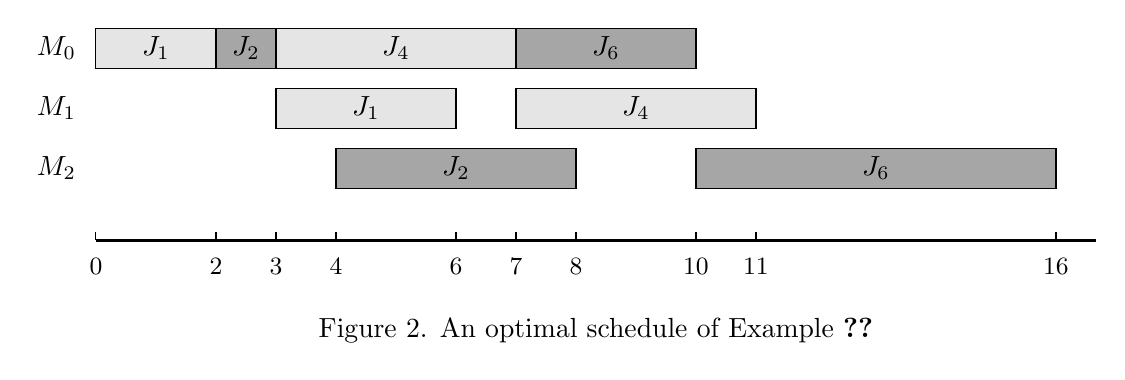
\begin{tikzpicture}[x=0.1in, y=0.2in]
                % machine index
                \node[anchor=east] at (-0.5,7) {$M_0$};
                \node[anchor=east] at (-0.5,5.5) {$M_1$};
                \node[anchor=east] at (-0.5,4) {$M_2$};
                
                % job on M_0
                \draw[fill=gray!20] (0,6.5) rectangle (6,7.5) node[midway] {$J_1$};
                \draw[fill=gray!70] (6,6.5) rectangle (9,7.5) node[midway] {$J_2$};
                \draw[fill=gray!20] (9,6.5) rectangle (21,7.5) node[midway] {$J_4$};
                \draw[fill=gray!70] (21,6.5) rectangle (30,7.5) node[midway] {$J_6$};
                
                % job on M_1
                \draw[fill=gray!20] (9,5) rectangle (18,6) node[midway] {$J_1$};
                \draw[fill=gray!20] (21,5) rectangle (33,6) node[midway] {$J_4$};
                
                % job on M_2
                \draw[fill=gray!70] (12,3.5) rectangle (24,4.5) node[midway] {$J_2$};
                \draw[fill=gray!70] (30,3.5) rectangle (48,4.5) node[midway] {$J_6$};
                
                % x-axis
                \draw[thick] (0,2.2) -- (50,2.2);
                \foreach \x/\label in {0/0, 6/2, 9/3, 12/4, 18/6, 21/7, 24/8, 30/10, 33/11, 48/16} {
                    \draw (\x,2.2) -- (\x,2.4);
                    \node[below, font=\small] at (\x,2.0) {\label};
                }
                
                % caption
                \node[below] at (25,0.5) {Figure 2. An optimal schedule of Example \ref{EX-2.1}};
            \end{tikzpicture}
        \end{center}
        
        
        \subsection{An FPTAS for the $FF2(1, m) \mid \mid  \sum_{J_j \in \mathcal{X}} w_j$ problem}
        
        An algorithm ${\mathcal A}$ is called a $(1-\eta)$-\textit{approximation} algorithm for a maximization problem if, for any instance, ${\mathcal A}$ outputs a solution whose objective value is at least  $(1-\eta)$ times the optimal value, where $0 <\eta < 1$.  A set of algorithms $\{{\mathcal A}_{\epsilon}\}$ constitutes an \textit{FPTAS} if, for each fixed $0 < \epsilon <1$, ${\mathcal A}_{\epsilon}$ outputs a $(1-\epsilon)$-approximation solution with time complexity polynomial in both $1/{\epsilon}$ and the input size.
        By utilizing the technique of rounding the input data (\citealp{Sahni1976JACM}), we convert Algorithm $\mathbf{DP_1}$ into an FPTAS for the $FF2(1, m) \mid \mid \sum_{J_j \in \mathcal{X}} w_j$ problem when $m$ is fixed. One key point of this technique involves the determination of valid lower and upper bounds for the optimal objective value.
        
        To this end, consider an instance $\mathcal{I}$ of the $FF2(1, m) \mid \mid | \sum_{J_j \in \mathcal{X}} w_j$ problem. Let $(\mathcal{X}^{*}, \overline{\mathcal{X}^{*}})$ be an optimal partition of $\mathcal{I}$, and let $W^{*}$ denote its corresponding total weight of JIT jobs, i.e., $W^{*}=\sum_{J_j \in \mathcal{X}^{*}} w_j$.
        
        Moreover, for each $k=1, 2, \ldots, m$, define $\mathcal{I}_{res}^k$ as the $k$-\textit{restricted} instance of $\mathcal{I}$ in which only jobs belonging to $\mathcal{G}_k$ are considered. For each $k$, let $(\mathcal{X}_k^{*}, \overline{\mathcal{X}_k^{*}})$ be an optimal partition of $\mathcal{I}_{res}^k$, and let $W_k^{*}$ denote its corresponding total weight of JIT jobs, i.e., $W_k^{*}=\sum_{J_j \in \mathcal{X}_k^{*}} w_j$. 
        
        With respect to each $k=1, 2, \ldots, m$, define $\mathcal{X}^{(k)}=\mathcal{X}_k^{*}$,  $\overline{\mathcal{X}^{(k)}}=\mathcal{J} \setminus \mathcal{X}_k^{*}$,  $\mathcal{X}_{(k)}=\mathcal{X}^{*} \cap \mathcal{G}_k$ and $\overline{\mathcal{X}_{(k)}}=\mathcal{G}_k \setminus \mathcal{X}_{(k)}$. Due to the facts that all $(\mathcal{X}^{(1)}, \overline{\mathcal{X}^{(1)}}), (\mathcal{X}^{(2)}, \overline{\mathcal{X}^{(2)}}), \ldots, (\mathcal{X}^{(m)}, \overline{\mathcal{X}^{(m)}})$ are feasible partitions of $\mathcal{I}$, and $(\mathcal{X}_{(k)}, \overline{\mathcal{X}_{(k)}})$ is a feasible partition of $\mathcal{I}_{res}^k$ for $k=1, 2, \ldots, m$, it follows that 
        \begin{equation} \label{Eq-3.2.1}
            \max_{k=1, 2, \ldots, m}\{W_k^{*}\} \leq W^{*} \leq \sum_{j=1}^m W_k^{*} \leq m \max_{k=1, 2, \ldots, m}\{W_k^{*}\}.
        \end{equation}
        
        Note that any exact or approximation algorithm designed for the $F2 \mid \mid \sum_{J_j \in \mathcal{X}} w_j$ problem can be directly used to solve $\mathcal{I}_k^{res}$,  $k=1, 2, \ldots, m$. \cite{Elalouf2013JOS} provided an FPTAS for the $F2 \mid \mid \sum_{J_j \in \mathcal{X}} w_j$ problem with time complexity $O(n^3/\epsilon)$. For each $k=1, 2, \ldots, m$, by setting $\epsilon=\frac{1}{2}$, a  $\frac{1}{2}$-approximation schedule (referred to as $\sigma_k^{\frac{1}{2}}$) for $\mathcal{I}_{res}^k$ can be obtained  in $O(n_k^3)$ time through the application of the FPTAS provided by \cite{Elalouf2013JOS}, and let $W_k'$ be the objective value of this approximation solution. Then, we have 
        \begin{equation} \label{Eq-3.2.2}
            W_k' \leq W_k^{*} \leq 2 W_k', ~~ k=1, 2, \ldots, m.
        \end{equation}
        
        Define $W_{\mathrm{LB}}=\max\{W_k': k=1, 2, \ldots, m\}$. In view of \eqref{Eq-3.2.1} and \eqref{Eq-3.2.2}, we derive  
        \begin{equation} \label{Eq-3.2.3}
            W_{\mathrm{LB}} \leq W^{*} \leq 2m W_{\mathrm{LB}}.
        \end{equation} 
        
        The following algorithm (referred to as $\mathbf{DP_{\epsilon}}$) forms an FPTAS for the $FF2(1, m)\mid \mid \sum_{J_j \in \mathcal{X}} w_j$ problem. 
        
        \begin{algorithm}[tbp] 
            \small
            \linespread{1.2}\selectfont
            \SetAlgoLined
            \DontPrintSemicolon
            \hrule 
            \vspace{0.1cm}
            \textbf{Algorithm $\mathbf{DP_{\epsilon}}$:} An FPTAS for the $FF2(1, m)\mid \mid \sum_{J_j \in \mathcal{X}} w_j$ problem
            \vspace{0.1cm}
            \hrule 
            \vspace{0.1cm}
            
            %\LinesNumbered 
            \KwIn{$\mathcal{J}$, $\epsilon$, $m$, $n$, $a_j$, $b_j$, $d_j$, $w_j$, $g_j$, $j=1, 2, \ldots, n$.}
            \vspace{0.1cm}
            
            \begin{description}
                \item[Step 1.] For each $k=1, 2, \ldots, m$, calculate the objective value $W_k'$ of the approximate schedule $\sigma_k^{\frac{1}{2}}$ for $\mathcal{I}_{res}^k$.  Set $W_{\mathrm{LB}}=\max\{W_k': k=1, 2, \ldots, m\}$.
                
                \item[Step 2.] Set $\Delta^{\#}=\frac{\epsilon W_{\mathrm{LB}}}{n}$. Define a new instance $\mathcal{I}^{\#}$ from the original instance $\mathcal{I}$ in which each job $J_j$ is replaced by a counterpart $J_j^{\#}$ such that $w_j^{\#}=\lfloor \frac{w_j}{\Delta^{\#}} \rfloor$, while all other parameters remain unchanged.
                
                \item[Step 3.] Apply Algorithm $\mathbf{DP_1}$ with the elimination rule (R-2) to the scaled instance $\mathcal{I}^{\#}$ and obtain its optimal schedule $\pi_{\#}$. Denote the corresponding set of JIT jobs by $\mathcal{X}_{\#}$ and its total weight by $W^{\#}$.
                
                \item[Step 4.] Convert the schedule $\pi_{\#}$ for $\mathcal{I}^{\#}$ back to a schedule $\pi_{\epsilon}$ for $\mathcal{I}$. Denote the corresponding set of JIT jobs by $\mathcal{X}_{\epsilon}$ and its total weight by $W^{\epsilon}$.
            \end{description}
            \KwOut{An approximate schedule $\pi_{\epsilon}$, along with its corresponding JIT job set $\mathcal{X}_{\epsilon}$ and total weight $W^{\epsilon}$.}
            \vspace{0.1cm}
            \hrule 
        \end{algorithm}
        
        
        \begin{lemma} \label{Lem-3.4}
            For any $0 < \epsilon <1$, Algorithm $\mathbf{DP_{\epsilon}}$ outputs a feasible schedule $\pi_{\epsilon}$ with $W^{\epsilon} \geq (1-\epsilon) W^{*}$
        \end{lemma}
        
        \noindent\textbf{Proof.} Since the two instances $\mathcal{I}^{\#}$ and $\mathcal{I}$ differ only in job weights, the feasibility of $\pi_{\#}$ for $\mathcal{I}^{\#}$ implies that $\pi_{\epsilon}$ is feasible for $\mathcal{I}$. Observe that $J_j \in  \mathcal{X}_{\epsilon}$ if and only if $J_j^{\#} \in \mathcal{X}_{\#}$. Since $\lfloor \theta \rfloor \leq \theta$ holds for any real $\theta$, we have 
        \begin{equation} \label{Eq-R1}
            W^{\epsilon} = \sum_{J_j \in \mathcal{X}_{\epsilon}} w_j 
            = \Delta^{\#} \sum_{J_j \in \mathcal{X}_{\epsilon}} \frac{w_j}{\Delta^{\#}} 
            \geq \Delta^{\#} \sum_{J_j^{\#} \in \mathcal{X}_{\#}} \lfloor \frac{w_j}{\Delta^{\#}} \rfloor
            = \Delta^{\#} \sum_{J_j^{\#} \in \mathcal{X}_{\#}} w_j^{\#}= \Delta^{\#} W^{\#}.
        \end{equation}
        
        Define $\mathcal{X}^{*}_{\#}=\{J_j^{\#}: J_j \in \mathcal{X}^{*}\}$ and $\overline{\mathcal{X}^{*}_{\#}}=\{J_j^{\#}: J_j \in \overline{\mathcal{X}^{*}}\}$. Since $(\mathcal{X}^{*}, \overline{\mathcal{X}^{*}})$ is an optimal partition of $\mathcal{I}$, it follows that $(\mathcal{X}^{*}_{\#}, \overline{\mathcal{X}^{*}_{\#}})$ is a feasible partition of $\mathcal{I}^{\#}$. From the facts that $\lfloor \theta \rfloor \geq \theta-1$ and $\pi_{\#}$ is an optimal schedule for $\mathcal{I}^{\#}$, we have 
        \begin{equation} \label{Eq-R2}
            W^{\#}=\sum_{J_j^{\#} \in \mathcal{X}_{\#}} w_j^{\#} 
            \geq \sum_{J_j^{\#} \in \mathcal{X}^{*}_{\#}} w_j^{\#}
            \geq \sum_{J_j^{\#} \in \mathcal{X}^{*}_{\#}}(\frac{w_j}{\Delta^{\#}}-1) 
            = \sum_{J_j \in \mathcal{X}^{*}}\frac{w_j}{\Delta^{\#}}-|\mathcal{X}^{*}|.
        \end{equation}
        
        Note that $\Delta^{\#}=\frac{\epsilon W_{\mathrm{LB}}}{n}$ and $|\mathcal{X}^{*}| \leq n$. Then combining \eqref{Eq-3.2.3}, \eqref{Eq-R1} and \eqref{Eq-R2}, we have
        \begin{equation} \label{Eq-R3}
            W^{\epsilon} \geq \Delta^{\#} W^{\#}
            \geq \sum_{J_j \in \mathcal{X}^{*}} w_j-|\mathcal{X}^{*}|\Delta^{\#} \geq W^{*}-n \Delta^{\#}=W^{*}-\epsilon W_{\mathrm{LB}} \geq (1-\epsilon) W^{*}.
        \end{equation}
        \hfill$\Box$
        
        
        \begin{theorem} \label{The-3.2}
            For fixed $m$, there exists an FPTAS for the $FF2(1, m)\mid \mid \sum_{J_j \in \mathcal{X}} w_j$ problem that runs in $O(n^2 (\Pi_{k=1}^m n_k)/{\epsilon})$ time.
        \end{theorem}
        
        \noindent\textbf{Proof.} By Lemma \ref{Lem-3.4}, it suffices to estimate the time complexity of Algorithm $\mathbf{DP_{\epsilon}}$. In Step 1, computing $W_{\mathrm{LB}}$ requires $O(\sum_{k=1}^m n_k^3)=O(n^3)$ time, as each $W_k'$ can be calculated in $O(n_k^3)$ time for $k=1, 2, \ldots, m$. In Step 2, constructing the scaled instance needs $O(n)$ time. Based on the elimination rule (R-2) and the bound \eqref{Eq-3.2.3}, the number of distinct $W$ values is at most $\lfloor \frac{2m W_{\mathrm{LB}}}{\Delta^{\#}}\rfloor \leq \frac{2mn}{\epsilon}=O(\frac{n}{\epsilon})$. Hence, by Theorem \ref{T-3.1}, Step 3 runs in $O(\frac{n^2 \Pi_{k=1}^m n_k}{\epsilon})$ time. In Step 4, generating schedule $\pi_{\#}$ requires $O(n \log n)$ time. Hence, the entire algorithm runs in $O(\frac{n^2 \Pi_{k=1}^m n_k}{\epsilon})$ time. \hfill$\Box$ 
        
        
        \section{The $FF2(m, 1)\mid \mid \sum_{J_j \in \mathcal{X}} w_j$ problem}
        
        In this section, we first prove two $\mathcal{NP}$-hardness results for the $FF2(m, 1)\mid \mid \sum_{J_j \in \mathcal{X}} w_j$ problem, and then design an exact pseudo-polynomial DP algorithm for fixed $m$.
        
        \subsection{Complexity analysis of the $FF2(m, 1) \mid \mid |\mathcal{X}|$ problem}
        
        In contrast to the $FF2(1, m)\mid \mid |\mathcal{X}|$ problem, which is polynomially solvable for fixed $m$ (Corollary \ref{C-3.2}), the $FF2(m, 1) \mid \mid |\mathcal{X}|$ problem proves to be much harder. We establish two $\mathcal{NP}$-hardness results for the case where $b_j=1$ for $j = 1, 2, \ldots, n$: (i) it is strongly $\mathcal{NP}$-hard for arbitrary $m$; (ii) it is ordinarily $\mathcal{NP}$-hard for $m = 2$.
        
        \begin{theorem} \label{T-4.1}
            When $m$ is arbitrary, the $FF2(m, 1) \mid b_j=1 \mid |\mathcal{X}|$ problem is strongly $\mathcal{NP}$-hard. 
        \end{theorem}
        
        \noindent \textbf{Proof.} To prove the result, we present a polynomial-time reduction from the strongly $\mathcal{NP}$-complete \emph{3-Partition} problem (\citealp{Garey1979computer}). 
        
        \textbf{3-Partition:} Given $3r$ positive integers $q_1, q_2, \ldots, q_{3r}$ and an integer $Q$ satisfying $\sum_{j=1}^{3r} q_j=r Q$ and $\frac{Q}{4} < q_j < \frac{Q}{2}$ for each $j=1, 2, \ldots, 3r$, is there a partition of the index set $\mathcal{S}=\{1, 2, \ldots, 3r\}$ into $r$ disjoint sets $\mathcal{S}_1, \mathcal{S}_2, \ldots, \mathcal{S}_r$ satisfying $\sum_{j \in \mathcal{S}_k} q_j =Q$ and $|\mathcal{S}_k|=3$ for each $k=1, 2, \ldots, r$?
        
        From an arbitrary 3-Partition instance $\mathcal{I}_{3\text{-}par}$, we create an instance $\mathcal{I}_{sch}$ of the $FF2(m, 1) \mid  b_j=1 \mid |\mathcal{X}|$ problem as follows: 
        \begin{itemize}
            \item There are $m=r$ parallel dedicated machines at stage 1 and a single common bottleneck machine at stage 2.
            
            \item There are $n=3 r^2$ jobs that are partitioned into $m$ disjoint groups, where $\mathcal{G}_k=\{J_{3(k-1)r+1}, J_{3(k-1)r+2}, \ldots, J_{3kr}\}$ for $k=1, 2, \ldots, r$.
            
            \item The job parameters are $a_{3(k-1)r+j}=3r q_j$, $b_{3(k-1)r+j}=1$, $d_{3(k-1)r+j}=3rQ+j$, and $w_{3(k-1)r+j}=1$ for each $j=1, 2, \ldots, 3r$ and $k=1, 2, \ldots, r$.
            
            \item The threshold value of the objective function is $Y=3r$.
            
            \item The decision variant associated with $\mathcal{I}_{sch}$ asks to verify the existence of a feasible schedule containing at least $Y$ JIT jobs.	
        \end{itemize}
        
        We show that $\mathcal{I}_{sch}$ has a feasible schedule with at least $Y$ JIT jobs if and only if $\mathcal{I}_{3\text{-}par}$ has a solution.  
        
        Assume that $\mathcal{I}_{3\text{-}par}$ has a solution $(\mathcal{S}_1, \mathcal{S}_2, \ldots, \mathcal{S}_r)$. This means that $\sum_{j \in \mathcal{S}_k} q_j=Q$ and $|\mathcal{S}_k|=3$ for each $k=1, 2, \ldots, r$. Define $\mathcal{X}=\mathcal{X}_1 \cup \mathcal{X}_2 \cup \cdots \cup \mathcal{X}_r$, where $\mathcal{X}_k=\{J_{3(k-1)r+j}: j \in \mathcal{S}_k\}$ for $k=1, 2, \ldots, r$. Clearly, $|\mathcal{X}_k|=3$ holds for every $k$. A feasible schedule $\sigma$ corresponding to $\mathcal{X}$ can be constructed as follows. For each $k=1, 2, \ldots, r$, the jobs in $\mathcal{X}_k$ are first processed on $M_k$ during the interval $[0, 3rQ]$. Then, for each $j=1, 2, \ldots, 3r$, if $j \in \mathcal{I}_k$, then job $J_{3(k-1)r+j}$ is scheduled on $M_0$ in the interval $[3rQ+j-1, 3rQ+j]$. Since $|\mathcal{X}|=3r=Y$, $\sigma$ contains exactly $Y$ JIT jobs and is feasible.
        
        Conversely, assume that $\mathcal{I}_{sch}$ has a feasible schedule $\sigma$ with at least $3r$ JIT jobs.
        Let $\mathcal{X}=\{J_j: C_j(\sigma)=d_j, j=1, 2, \ldots, 3r^2\}$ be the set of JIT jobs in $\sigma$.
        By assumption, $|\mathcal{X}| \geq 3r$. Define $\mathcal{X}_k = \mathcal{X} \cap \mathcal{G}_k$ for each $k=1, 2, \ldots, r$. Since $\mathcal{I}_{sch}$ has $3r$ distinct due dates and at most one job can be completed exactly on each due date in any feasible schedule, it follows that $|\mathcal{X}| \leq 3r$.
        Consequently,
        \begin{equation}\label{E-A.1}
            |\mathcal{X}_1|+|\mathcal{X}_2|+\cdots+|\mathcal{X}_r|=|\mathcal{X}|=3r.
        \end{equation}
        
        For each $k=1, 2, \ldots, r$, define $\mathcal{S}_k=\{j: J_{3(k-1)r+j} \in \mathcal{X}_k\}$.
        Then, we obtain
        \begin{equation}\label{E-A.2}
            \mathcal{S}_1 \cup \mathcal{S}_2 \cup \cdots \cup \mathcal{S}_r \subseteq \{1, 2, \ldots, 3r\}=\mathcal{S}
        \end{equation}
        and
        \begin{equation}\label{E-A.3}
            |\mathcal{S}_k| = |\mathcal{X}_k|, ~~ k=1, 2, \ldots, r.
        \end{equation}
        
        Observe that if $\mathcal{S}_u \cap \mathcal{S}_v \not=\emptyset$ for some $1 \leq u < v \leq r$, then for any $i \in \mathcal{S}_u \cap \mathcal{S}_v$, both jobs $J_{3(u-1)r+i}$ and $J_{3(v-1)r+i}$ would be JIT  in $\sigma$. This is impossible because they share the same due date $3rQ+i$. Therefore,
        \begin{equation}\label{E-A.4}
            \mathcal{S}_u \cap \mathcal{S}_v=\emptyset ~\mathrm{for ~each} ~ 1 \leq u < v \leq r.
        \end{equation}
        
        In view of \eqref{E-A.1}-\eqref{E-A.4}, it follows that $(\mathcal{S}_1, \mathcal{S}_2, \ldots, \mathcal{S}_r)$ forms a partition of $\mathcal{S}$. Hence,
        \begin{equation}\label{E-A.5}
            \sum_{j \in \mathcal{S}_1} q_j + \sum_{j \in \mathcal{S}_2} q_j + \cdots + \sum_{j \in \mathcal{S}_r} q_j
            =\sum_{j \in \mathcal{S}} q_j=\sum_{j=1}^{3r} q_j=rQ.
        \end{equation}
        
        Because the largest due date among all jobs in $\mathcal{X}$ is at most $d_{\max}=3rQ+3r$ and $b_j=1$ for each $j=1, 2, \ldots, 3r^2$, we have
        \begin{equation}\label{E-A.6}
            \sum_{J_j \in \mathcal{X}_k} a_j+1 = 3r \sum_{j \in \mathcal{S}_k} q_j+1 \leq d_{\max}= 3rQ+3r, ~ k=1, 2, \ldots, r.
        \end{equation}
        
        Simplifying \eqref{E-A.6} gives
        \begin{equation}\label{E-A.7}
            \sum_{j \in \mathcal{S}_k} q_j \leq Q, ~ k=1, 2, \ldots, r.
        \end{equation}
        
        Combining \eqref{E-A.5} and \eqref{E-A.7}, we have 
        \begin{equation}\label{E-A.8}
            \sum_{j \in \mathcal{S}_k} q_j =Q, ~ k=1, 2, \ldots, r. 
        \end{equation}
        
        Given that $\frac{Q}{4} < q_j < \frac{Q}{2}$ for each $j=1, 2, \ldots, 3r$, \eqref{E-A.8} implies that each $\mathcal{S}_k$ must contain exactly three elements, i.e., 
        \begin{equation}\label{E-A.9}
            |\mathcal{S}_k|=3, ~ k=1, 2, \ldots, r.
        \end{equation}	
        
        In view of \eqref{E-A.8}-\eqref{E-A.9}, $(\mathcal{S}_1, \mathcal{S}_2, \ldots, \mathcal{S}_r)$ constitutes a solution to $\mathcal{I}_{3\text{-}par}$.  \hfill$\Box$\\
        
        %\begin{rem}\label{R-A.1}
        %Theorem \ref{T-4.1} implies that a pseudo-polynomial-time algorithm and an FPTAS cannot be constructed for the $FF2(m, 1) \mid \mid \sum_{J_j \in \mathcal{X}} w_j$ problem when $m$ is arbitrary.
        %\end{rem}
        
        
        
        \begin{theorem} \label{T-4.2}
            The $FF2(2, 1) \mid b_j=1 \mid |\mathcal{X}|$ problem is ordinarily $\mathcal{NP}$-hard.
        \end{theorem}
        
        \noindent \textbf{Proof.} To prove the result, we present a polynomial-time reduction from the ordinarily  $\mathcal{NP}$-complete \emph{Partition} problem (\citealp{Garey1979computer}).
        
        \textbf{Partition:} Given $r$ positive integers $q_1, q_2, \ldots, q_r$ and an integer $Q$ with $\sum_{j=1}^r q_j=2Q$, is there a partition of the index set $\mathcal{S}=\{1, 2, \ldots, r\}$ into two disjoint sets $\mathcal{S}_1$ and $\mathcal{S}_2$ satisfying $\sum_{j \in \mathcal{S}_1} q_j = \sum_{j \in \mathcal{S}_2} q_j=Q$?
        
        From an arbitrary Partition instance $\mathcal{I}_{par}$, we create an instance $\mathcal{I}_{sch}$ of the $FF2(2, 1) \mid b_j=1 \mid |\mathcal{X}|$ problem  as follows: 
        \begin{itemize}
            \item There are $m=2$ parallel dedicated machines at stage 1 and a single common bottleneck machine at stage 2. 
            
            \item There are $n=2r$ jobs that are partitioned into two disjoint groups, where $\mathcal{G}_1=\{J_1, J_2, \ldots, J_r\}$ and $\mathcal{G}_2=\{J_{r+1}, J_{r+2}, \ldots, J_{2r}\}$.
            
            \item The job parameters are $a_j=a_{r+j}=r q_j$, $b_j=b_{r+j}=1$, $d_j=d_{r+j}=rQ+j$, and $w_j=w_{r+j}=1$ for each $j=1, 2, \ldots, r$.
            
            \item The threshold value of the objective function is $Y=r$.
            
            \item The decision variant associated with $\mathcal{I}_{sch}$ asks to verify the existence of a feasible schedule containing at least $Y$ JIT jobs.
        \end{itemize}
        
        We show that $\mathcal{I}_{sch}$ has a feasible schedule with at least $Y$ JIT jobs if and only if $\mathcal{I}_{par}$ has a solution.
        
        Assume that $\mathcal{I}_{par}$ has a solution $(\mathcal{S}_1, \mathcal{S}_2)$ with $\sum_{j \in \mathcal{S}_1} q_j = \sum_{j \in \mathcal{S}_2} q_j=Q$. Define $\mathcal{X}_1=\{J_j: j \in \mathcal{S}_1\}$ and $\mathcal{X}_2=\{J_{r+j}: j \in \mathcal{S}_2\}$. A feasible schedule $\sigma$ corresponding to $\mathcal{X}_1 \cup \mathcal{X}_2$ for $\mathcal{I}_{sch}$ is constructed as follows. For each $k=1, 2$, the jobs in $\mathcal{X}_k$ are first processed on $M_k$ during the  interval $[0, rQ]$. Then, for each $j=1, 2, \ldots, r$, either $J_j$ (if $j \in \mathcal{S}_1$) or $J_{r+j}$ (if $j \in \mathcal{S}_2$) is scheduled on $M_0$ in the interval $[rQ+j-1, rQ+j]$. Since $|\mathcal{X}_1 \cup \mathcal{X}_2|=r=Y$, $\sigma$ contains exactly $Y$ jobs and is feasible.
        
        Conversely, assume that $\mathcal{I}_{sch}$ has a feasible schedule $\sigma$ with at least $r$ JIT jobs. Let $\mathcal{X}_1=\{J_j \in \mathcal{G}_1: C_j(\sigma)=d_j\}$ and $\mathcal{X}_2=\{J_j \in \mathcal{G}_2: C_j(\sigma)=d_j\}$ be the sets of JIT jobs in $\mathcal{G}_1$ and $\mathcal{G}_2$ in $\sigma$, respectively. By assumption, $|\mathcal{X}_1|+|\mathcal{X}_2| \geq r$.
        Define $\mathcal{S}_1=\{j: J_j \in \mathcal{X}_1\}$ and $\mathcal{S}_2=\{j: J_{r+j} \in \mathcal{X}_2\}$. Since $\mathcal{I}_{sch}$ has $r$ distinct due dates and at most one job can be completed exactly on each due date in any feasible schedule, it follows that $|\mathcal{X}_1|+|\mathcal{X}_2| \leq r$. Consequently, we have 
        \begin{equation}\label{E-C.0}
            |\mathcal{S}_1|+|\mathcal{S}_2|=|\mathcal{X}_1|+|\mathcal{X}_2| =r= |\mathcal{S}|.
        \end{equation}
        Moreover, since $d_j=d_{r+j}=rQ+j$ for each $j=1, 2, \ldots, r$, we have $\mathcal{S}_1 \cap \mathcal{S}_2=\emptyset$. In view of \eqref{E-C.0}, this further implies that $\mathcal{S}_1 \cup \mathcal{S}_2=\mathcal{S}$.
        As a consequence,  
        \begin{equation}\label{E-C.1}
            \sum_{j \in \mathcal{S}_1} q_j + \sum_{j \in \mathcal{S}_2} q_j =\sum_{j \in \mathcal{S}} q_j=2Q.
        \end{equation}
        
        Because the largest due date among all jobs in $\mathcal{X}_1 \cup \mathcal{X}_2$ is $d_{\max}=rQ+r$ and $b_j=1$ for each $j=1, 2, \ldots, 2r$, we have 
        \begin{equation}\label{E-C.2}
            \sum_{J_j \in \mathcal{X}_k} a_j+1 = r \sum_{J_j \in \mathcal{S}_k} q_j+1 \leq d_{\max}= rQ+r, ~ k=1, 2.
        \end{equation}
        
        Simplifying \eqref{E-C.2} gives 
        \begin{equation}\label{E-C.3}
            \sum_{j \in \mathcal{S}_k} q_j \leq Q, ~ k=1, 2.
        \end{equation}
        
        Combining \eqref{E-C.1} and \eqref{E-C.3}, we have $\sum_{j \in \mathcal{S}_1} q_j = \sum_{j \in \mathcal{S}_2} q_j=Q$. Consequently, $(\mathcal{S}_1, \mathcal{S}_2)$ constitutes a solution to $\mathcal{I}_{par}$. \hfill$\Box$ 
        
        \subsection{A DP algorithm for the $FF2(m, 1) \mid \mid |\sum_{J_j \in \mathcal{X}} w_j$ problem}
        
        Before presenting our DP algorithm for the $FF2(m, 1)\mid \mid \sum_{J_j \in \mathcal{X}} w_j$ problem, we first characterize several structural properties of an optimal schedule. Similar to the analysis preceding Lemma \ref{L-3.1}, the following result holds.
        
        \begin{lemma} \label{L-4.1}
            For the $FF2(m, 1)\mid \mid \sum_{J_j \in \mathcal{X}} w_j$ problem, an optimal schedule exists such that each machine $M_k$ ($k=1, 2, \ldots, m$) processes jobs continuously without idle times.
        \end{lemma}
        
        As shown in \cite{ChoiYoon2007JOS}, the $F2\mid \mid \sum_{J_j \in \mathcal{X}} w_j$ problem admits an optimal schedule where the JIT jobs are processed in EDD order on both machines. We can generalize the result to the $FF2(m, 1)\mid \mid \sum_{J_j \in \mathcal{X}} w_j$ problem for arbitrary $m$.
        
        \begin{lemma} \label{L-4.2}
            For the $FF2(m, 1)\mid \mid \sum_{J_j \in \mathcal{X}} w_j$ problem, an optimal schedule exists such that: (i) on the common bottleneck machine $M_0$, the JIT jobs in $\mathcal{X}$ are processed in EDD order; and (ii) on each dedicated machine $M_k$ ($k=1, 2, \ldots, m$), the JIT jobs in $\mathcal{X} \cap \mathcal{G}_k$ are processed in EDD order.
        \end{lemma}
        
        \noindent \textbf{Proof.} Owing to the facts that all JIT jobs must be completed exactly on their due dates and no two jobs can overlap on the same machine, the JIT jobs in $\mathcal{X}$ must be sequenced on $M_0$ in EDD order in any optimal schedule. This establishes property (i).
        
        Next, let $\sigma$ be an optimal schedule satisfying property (i) but violating property (ii). Then, there exist a machine index $k \in \{1, 2, \ldots, m\}$ and two job indices $u$ and $v$ such that $J_u, J_v \in \mathcal{X} \cap \mathcal{G}_k$, $d_u > d_v$, and $J_u$ is sequenced just before $J_v$ on $M_k$ in $\sigma$. An alternative schedule $\sigma'$ can be created from
        $\sigma$ by swapping positions of $J_u$ and $J_v$ on $M_k$. This swapping does not change the start time of any JIT job on $M_0$. By applying this swapping procedure to each $M_k$ ($k=1, 2, \ldots, m$) a finite number of times, we obtain an optimal schedule satisfying both properties (i) and (ii). \hfill$\Box$\\ 
        
        Owing to Lemmas \ref{L-4.1} and \ref{L-4.2}, an optimal schedule for the $FF2(m, 1) \mid \mid |\sum_{J_j \in \mathcal{X}} w_j$ problem can be fully determined by an optimal partition of $\mathcal{J}$ into a set $\mathcal{X}$ of JIT jobs and its complement $\overline{\mathcal{X}}=\mathcal{J} \setminus \mathcal{X}$ of rejected jobs. To simplify the presentation, the $n$ jobs in $\mathcal{J}$ are assumed to be numbered in EDD order throughout this section, i.e.,
        \begin{equation}\label{Eq-4.3.1}
            d_1 \leq d_2 \leq \cdots \leq d_n,
        \end{equation}
        where ties are broken arbitrarily. 
        
        For $j=1, 2, \ldots, n$, let $\mathcal{J}_j=\{J_1, J_2, \ldots, J_j\}$ denote the set of the first $j$ jobs in  $\mathcal{J}$. We describe a DP approach for the $FF2(m, 1)\mid \mid \sum_{J_j \in \mathcal{X}} w_j$ problem. Consider a feasible partial schedule  on $\mathcal{J}_j$ that satisfies Lemmas \ref{L-4.1} and \ref{L-4.2} and includes $J_j$ as a JIT job. Denote by $\mathcal{X}_j$ the set of JIT jobs in this schedule and by $\overline{\mathcal{X}}_j$ its complement. Every such feasible partial schedule can be uniquely represented by an $(m+2)$-dimension tuple $(T_1, T_2, \ldots, T_m, W, \mathcal{X}_j)$, subject to the following conditions: 
        \begin{description}
            \item (D1) For each $k=1, 2, \ldots, m$, $T_k=\sum_{J_i \in \mathcal{X}_j \cap \mathcal{G}_k} a_i$ denotes the total processing time of JIT jobs in $\mathcal{X}_j \cap \mathcal{G}_k$ on $M_k$ (if $\mathcal{X}_j \cap \mathcal{G}_k=\emptyset$, define $T_k=0$);
            
            \item (D2) $W=\sum_{J_i \in \mathcal{X}_j} w_i$ denotes the total weight of JIT jobs in $\mathcal{X}_j$;
            
            \item (D3) $J_j$ is a JIT job, i.e., $J_j \in \mathcal{X}_j$.
        \end{description}
        From these definitions, we have: (i) for each $k=1, 2, \ldots, m$, $0 \leq T_k \leq \sum_{J_i \in \mathcal{J}_j \cap \mathcal{G}_k} a_i$; and (ii) $w_j \leq W \leq \sum_{i=1}^j w_i$. Note that (D1) means that the completion time of the last JIT job (if any) on $M_k$ is $T_k$; (D3) implies that $J_j$ is a JIT job and, by Lemma \ref{L-4.2}, it should be scheduled last on $M_0$. 
        
        For each $j=0, 1, \ldots, n$, let $\mathcal{H}_j$ be the set of all tuples corresponding to feasible partial schedules on $\mathcal{J}_j$ that satisfy conditions (D1)-(D3). To derive the tuple transition process, consider a tuple $(T'_1, T'_2, \ldots, T'_m, W', \mathcal{X}'_j) \in \mathcal{H}_j$ and let $\pi$ be a corresponding feasible partial schedule on $\mathcal{J}_j$. By definition, the set of JIT jobs in $\pi$ is $\mathcal{X}'_j$, $J_j$ is scheduled last on $M_0$, and its first operation' completion time on $M_{g_j}$ is exactly $T'_{g_j}$. Because $J_j$ is a JIT job, its second operation must be processed on $M_0$ within the interval $[d_j-b_j, d_j]$. This implies two conditions:  
        \begin{description}
            \item (D4) The first operation of $J_j$ on $M_{g_j}$ must be completed by time $d_j-b_j$, so $T'_{g_j} \leq d_j-b_j$.
            
            \item (D5) Any preceding JIT job (if any) on $M_0$ must finish by time $d_j-b_j$.
        \end{description}
        Let $J_i$ be the second-to-last JIT job processed on $M_0$ in $\pi$. By Lemma \ref{L-4.2} and condition (D5), we have $i=\arg_k \max\{J_k \in \mathcal{X}'_j \setminus \{J_j\}\}$ and $d_i \leq d_j-b_j$. By removing $J_j$ from $\pi$, we obtain a partial schedule $\pi'$ on $\mathcal{J}_i$. This schedule is feasible for $\mathcal{J}_i$, satisfies Lemmas \ref{L-4.1} and \ref{L-4.2}, and has $\mathcal{X}'_j \setminus \{J_j\}$ as its JIT job set. Consequently, the tuple corresponding to $\pi'$ is $(T'_1, T'_2, \ldots, T'_{g_j-1}, T'_{g_j}-a_j, T'_{g_j+1}, \ldots, T'_m, W'-w_j, \mathcal{X}'_j \setminus \{J_j\})$. Clearly, This tuple belongs to $\mathcal{H}_i$. The above discussion shows that every tuple in $\mathcal{H}_j$ can be generated from a tuple in $\mathcal{H}_i$ for some $i \in \{0, 1,  \ldots, j-1\}$.
        
        The algorithm is initialized with $\mathcal{H}_0=\{(T_1=0, T_2=0, \ldots, T_m=0, W=0, \mathcal{X}_0=\emptyset)\}$, which corresponds to a dummy schedule. In the $j$-th iteration ($1 \leq j \leq n$), the tuple set $\mathcal{H}_j$ is constructed dynamically from the previously generated sets $\mathcal{H}_0, \mathcal{H}_{1}, \ldots, \mathcal{H}_{j-1}$. For each $i=0, 1, \ldots, j-1$, let $\mathcal{H}_{j,i} \subseteq \mathcal{H}_j$ denote the subset of tuples in which the second-to-last JIT job on $M_0$ is $J_i$. Then for any feasible partial schedule on $\mathcal{J}_j$ that corresponds to a tuple in $\mathcal{H}_{j,i}$, the jobs $J_{i+1}, J_{i+2}, \ldots, J_{j-1}$ are rejected. As a consequence, for each tuple $(T_1, T_2, \ldots, T_m, W, \mathcal{X}_i) \in \mathcal{H}_i$, if 
        \begin{equation} \label{E-cond2}
            \max\{T_{g_j}+a_j, d_i\}+b_j \leq d_j,
        \end{equation} 
        then the tuple $(T_1, T_2, \ldots, T_{g_j-1}, T_{g_j}+a_j, T_{g_j+1}, \ldots, T_m, W+w_j, \mathcal{X}_i \cup \{J_j\})$ is added to $\mathcal{H}_{j,i}$. Condition \eqref{E-cond2} ensures that $J_j$ can be scheduled as a JIT job immediately after $J_i$ on $M_0$ in the partial schedule corresponding to the tuple $(T_1, T_2, \ldots, T_m, W, \mathcal{X}_i)$. This holds because $d_j-b_j$ is the required start time of $J_j$ on $M_0$ when it is a JIT job, while $\max\{T_{g_j}+a_j, d_i\}$ is its earliest possible start time on $M_0$. Once all subsets $\mathcal{H}_{j,i}$ have been constructed, the final set $\mathcal{H}_j$ is obtained by setting $\mathcal{H}_{j}=\mathcal{H}_{j,0} \cup \mathcal{H}_{j,1} \cup \cdots \cup \mathcal{H}_{j,j-1}$.
        
        In the process of constructing $\mathcal{H}_j$, multiple tuples of the form $(T_1, T_2, \ldots, T_m, W, \mathcal{X}_j)$ may arise that share the same values of $T_1, T_2, \ldots, T_m$. However, the following elimination rule shows that among all tuples in $\mathcal{D}_j$ having identical $(T_1, T_2, \ldots, T_m)$, all dominated ones can be safely removed, we preserve only the one with the largest $W$ value.
        
        
        \begin{lemma} \label{L-4.3}
            For any two tuples $(T_1, T_2, \ldots, T_m, W, \mathcal{X}_j)$ and $(T_1', T_2', \ldots, T_m', W', \mathcal{X}_j')$ in $\mathcal{H}_j$ with $T_k \leq T_k'$ for $k=1, 2, \ldots, m$ and $W \geq W'$, the latter tuple can be removed from $\mathcal{H}_j$.
        \end{lemma}
        
        \noindent \textbf{Proof.} The proof employs an argument analogous to that used in Lemma \ref{L-3.3}.  \hfill$\Box$\\
        
        The exact DP algorithm for the $FF2(m, 1)\mid \mid \sum_{J_j \in \mathcal{X}} w_j$ problem is presented in Algorithm $\mathbf{DP_2}$. It maintains $W_{\text{best}}$ and $\mathcal{X}_{\text{best}}$ to record the best total weight and the corresponding JIT job set found so far. Jobs are considered in the order given by \eqref{Eq-4.3.1}, and the sets $\mathcal{H}_1, \mathcal{H}_{2}, \ldots, \mathcal{H}_{n}$ are constructed iteratively. In each iteration, $W_{\text{best}}$ and $\mathcal{X}_{\text{best}}$ are updated accordingly, and dominated tuples are removed according to Lemma \ref{L-4.3}.
        
        \begin{algorithm}[tbp]
            \small
            \linespread{1.2}\selectfont
            \SetAlgoLined
            \DontPrintSemicolon
            \hrule 
            \vspace{0.1cm}
            \textbf{Algorithm $\mathbf{DP_2}$:} A DP algorithm for the $FF2(m, 1)\mid \mid \sum_{J_j \in \mathcal{X}} w_j$ problem
            \vspace{0.1cm}
            \hrule 
            \vspace{0.1cm}
            \LinesNumbered 
            \KwIn{$\mathcal{J}$, $m$, $n$, $a_j$, $b_j$, $d_j$, $w_j$, $g_j$, $j=1, 2, \ldots, n$.}
            
            \textbf{Step 1.} [Preprocessing] Renumber the jobs in $\mathcal{J}$ according to \eqref{Eq-4.3.1}. \;
            
            \textbf{Step 2.} [Initialization] Set ${\mathcal H}_0=\{(T_1=0, T_2=0, \ldots, T_m=0, W=0, \mathcal{X}_0=\emptyset)\}$, $\mathcal{H}_j=\emptyset$ for $j=1, 2, \ldots, n$, $W_{\text{best}}=0$, and $\mathcal{X}_{\text{best}}=\emptyset$. \hspace*{\algorithmicindent}%
            \hangindent=\dimexpr\algorithmicindent*2\relax% 
            
            \textbf{Step 3.} [Generation] Generate sets $\mathcal{H}_1$ to $\mathcal{H}_n$. \;
            
            {\For{$j=1$ \KwTo $n$}
                {
                    \For{$i=0$ \KwTo $j-1$}
                    { $\mathcal{H}_{j,i}=\emptyset$.\;
                        
                        \For{each tuple $(T_1, T_2, \ldots, T_m, W, \mathcal{X}_i) \in \mathcal{H}_i$}
                        { 	
                            \If{$\max\{T_{g_j}+a_j, d_i\}+b_j \leq d_j$}
                            {
                                $T'_{g_j} \gets T_{g_j} + a_j$, $W' \gets W + w_j$, $\mathcal{X}' \gets \mathcal{X}_i \cup \{J_j\}$ \;
                                
                                $\mathcal{H}_{j,i} \leftarrow \mathcal{H}_{j,i} \cup (T_1, T_2, \ldots, T_{g_j-1}, T'_{g_j}, T_{g_j+1}, \ldots, T_m, W', \mathcal{X}')$ \;
                                
                                \If{$W' > W_{\text{best}}$}
                                {$W_{\text{best}} \gets W'$, $\mathcal{X}_{\text{best}} \gets \mathcal{X}'$ \;}
                            }	
                        }
                    }
                    
                    [Merging] Set $\mathcal{H}_{j}=\mathcal{H}_{j,0} \cup \mathcal{H}_{j,1} \cup \cdots \cup \mathcal{H}_{j,j-1}$. \;
                    
                    [Elimination] Among all tuples in $\mathcal{H}_j$ with identical $(T_1, T_2, \dots, T_m)$,  retain only the one with the largest $W$ value. \hspace*{\algorithmicindent}% 
                    \hangindent=\dimexpr\algorithmicindent*2\relax%
                }
            } 
            
            \textbf{Step 4.} [Result] Set $W^{*}=W_{\text{best}}$, $\mathcal{X}^*=\mathcal{X}_{\text{best}}$, and construct an optimal schedule $\pi^{*}$ by sequencing the jobs in $\mathcal{X}^*$ according to Lemmas \ref{L-4.1} and \ref{L-4.2}. \hspace*{\algorithmicindent}%
            \hangindent=\dimexpr\algorithmicindent*2\relax%
            
            \KwOut{An optimal schedule $\pi^{*}$, along with its corresponding JIT job set $\mathcal{X}^*$ and total weight $W^*$.}  
            \vspace{0.1cm}
            \hrule 
        \end{algorithm} 
        
        \begin{theorem} \label{T-4.3}
            Algorithm $\mathbf{DP_2}$ solves the $FF2(m, 1)\mid \mid \sum_{J_j \in \mathcal{X}} w_j$ problem in $O(n^2 \Pi_{k=1}^m \Phi_k)$ time, where $\Phi_k=\sum_{J_j \in \mathcal{G}_k} a_j$ for $k=1, 2, \ldots, m$. When $m$ is fixed, it is pseudo-polynomial.
        \end{theorem}
        
        \noindent \textbf{Proof.} The correctness of Algorithm $\mathbf{DP_2}$ is guaranteed by the two facts: (i) it enumerates all tuples that correspond to optimal schedules satisfying Lemmas \ref{L-4.1} and \ref{L-4.2}; and (ii) only dominated tuples are removed during the elimination procedure, as justified by Lemma \ref{L-4.3}.
        
        We now analyze its time complexity. Step 1 performs a sorting operation, which takes $O(n\log n)$ time. The initialization in Step 2 requires $O(n)$ time. Note that for each tuple $(T_1, T_2, \ldots, T_m, W, \mathcal{X}_j) \in \mathcal{H}_j$, we have $0 \leq T_k \leq \sum_{J_i \in \mathcal{J}_j \cap \mathcal{G}_k} a_i \leq \Phi_k$ for each $k=1, 2, \ldots, m$. In the $j$-th generation (lines 5-18) of Step 3, the elimination procedure ensures at most $O(\Pi_{k=1}^m \Phi_k)$ distinct tuples remain in $\mathcal{H}_j$. Consequently, $|\cup_{i=0}^{j-1} \mathcal{H}_i| \leq j \Pi_{k=1}^m \Phi_k$. Moreover, each state in $\mathcal{H}_i$ ($0 \leq i \leq j-1$) can generate at most one new state in $\mathcal{H}_j$. Thus, $\mathcal{H}_j$ can be constructed in $O(j \Pi_{k=1}^m \Phi_k)$ time. Summing over all $n$ generations in Step 3 gives an overall time of $O(n^2 \Pi_{k=1}^m \Phi_k)$. Step 4 constructs an optimal schedule in $O(n \log n)$ time. Therefore, the entire algorithm runs in $O(n^2 \Pi_{k=1}^m \Phi_k)$ time. \hfill$\Box$\\
        
        Note that when jobs in $\mathcal{G}_k$ have group-dependent and job-independent processing times on $M_k$ at stage 1 (i.e., $a_j=a^k$ for $J_j \in \mathcal{G}_k$), the number of distinct $T_k$ values in any tuple $(T_1, T_2, \ldots, T_m, W, \mathcal{X}_j) \in \mathcal{H}_j$ is bounded by $n_k$. Consequently, Theorem \ref{T-4.3} leads to the following corollary. 
        
        \begin{cor} \label{C-4.1}
            The $FF2(m, 1)\mid a_j=a^{g_j} \mid \sum_{J_j \in \mathcal{X}} w_j$ problem can be solved in $O(n^2 \Pi_{k=1}^m n_k)$ time, which is polynomial for fixed $m$.
        \end{cor}
        
        \begin{exam} \label{Ex-4.1}
            Consider a 6-job instance of the $FF2(2, 1)\mid \mid \sum_{J_j \in \mathcal{X}} w_j$ problem, with job parameters listed in Table \ref{Ta-4.1}.
        \end{exam}
        
        \begin{table}[htpb]
            \footnotesize
            \caption{Job parameters for Example \ref{Ex-4.1}} \label{Ta-4.1} 
            \begin{center}
                \begin{tabular}{c|cccccc}
                    $J_j$   & $J_1$ & $J_2$ & $J_3$ & $J_4$  & $J_5$ & $J_6$ \\ \hline
                    $a_j$   & 2 & 4  & 3 & 3 & 1 & 6   \\
                    $b_j$   & 3 & 4  & 3 & 2 & 4 & 5 \\
                    $d_j$   & 6 & 10  & 12 & 13 & 17 & 19 \\
                    $w_j$   & 3 & 4  & 5 & 6 & 7 & 5 \\
                    $g_j$   & 1 & 2  & 1 & 1 & 2 & 2 \\ \hline
                \end{tabular}
            \end{center}
        \end{table}
        
        Using Algorithm $\mathbf{DP_2}$, we get an optimal schedule shown in Figure 3. The corresponding JIT set is $\mathcal{X}^{*}=\{J_1, J_2, J_4, J_5\}$, with a total weight of 20. Because Algorithm $\mathbf{DP_2}$ follows a computational framework analogous to that of Algorithm $\mathbf{DP_1}$, its detailed calculations are omitted here. 
        \begin{center}
            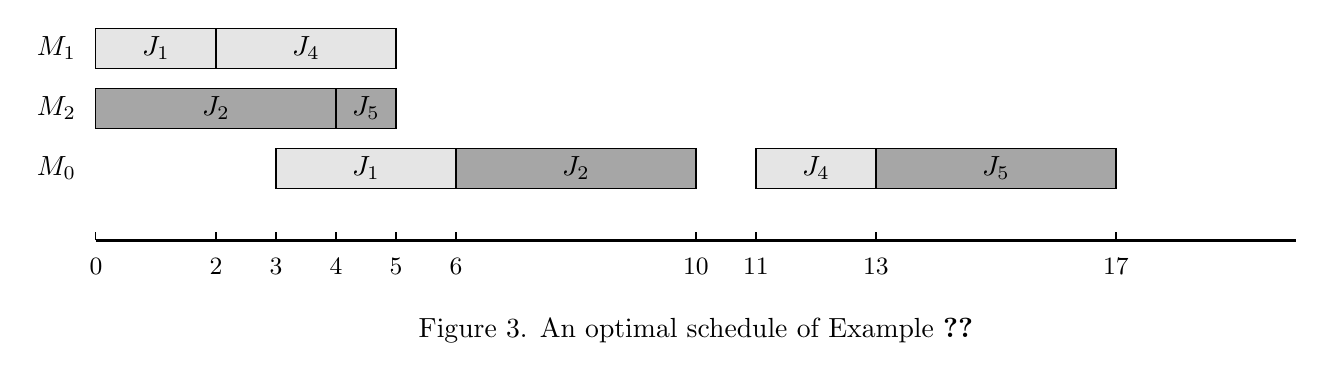
\begin{tikzpicture}[x=0.1in, y=0.2in]
                % machine index
                \node[anchor=east] at (-0.5,7) {$M_1$};
                \node[anchor=east] at (-0.5,5.5) {$M_2$};
                \node[anchor=east] at (-0.5,4) {$M_0$};
                
                % job on M_1
                \draw[fill=gray!20] (0,6.5) rectangle (6,7.5) node[midway] {$J_1$};
                \draw[fill=gray!20] (6,6.5) rectangle (15,7.5) node[midway] {$J_4$};
                
                % job on M_2
                \draw[fill=gray!70] (0,5) rectangle (12,6) node[midway] {$J_2$};
                \draw[fill=gray!70] (12,5) rectangle (15,6) node[midway] {$J_5$};
                
                % job on M_0
                \draw[fill=gray!20] (9,3.5) rectangle (18,4.5) node[midway] {$J_1$};
                \draw[fill=gray!70] (18,3.5) rectangle (30,4.5) node[midway] {$J_2$};
                \draw[fill=gray!20] (33,3.5) rectangle (39,4.5) node[midway] {$J_4$};
                \draw[fill=gray!70] (39,3.5) rectangle (51,4.5) node[midway] {$J_5$};
                
                % x-axis
                \draw[thick] (0,2.2) -- (60,2.2);
                \foreach \x/\label in {0/0, 6/2, 9/3, 12/4, 15/5, 18/6, 30/10, 33/11, 39/13, 51/17} {
                    \draw (\x,2.2) -- (\x,2.4);
                    \node[below, font=\small] at (\x,2.0) {\label};
                }
                
                % caption
                \node[below] at (30,0.5) {Figure 3. An optimal schedule of Example \ref{Ex-4.1}};
            \end{tikzpicture}
        \end{center}
        
        
        \section{Numerical study}
        
        To evaluate the performance of the DP algorithms designed in Sections 3 and 4, we conduct a series of computational experiments. The Matlab programs were executed on a PC with a 12th Generation Intel(R) Core(TM) i7-1260P CPU (2.10 GHz) and 16 GB of RAM.
        
        Given the high computational complexity of Algorithms $\mathbf{DP_1}$, $\mathbf{DP_{\epsilon}}$, and $\mathbf{DP_2}$, the parameter sets were systematically sampled based on the following assumptions:
        \begin{description}
            \item[(1)] Number of parallel dedicated machines: $m \in \{2, 3\}$.
            
            \item[(2)] Number of jobs: For the $FF2(1, m)\mid \mid \sum_{J_j \in \mathcal{X}} w_j$ problem, $n \in \{40, 80, \ldots, 400\}$ when $m=2$, and $n \in \{30, 60, \ldots, 180\}$ when $m=3$, where $n_i=n/m$ for $i=1, 2, \ldots, m$. For the $FF2(m, 1)\mid \mid \sum_{J_j \in \mathcal{X}} w_j$ problem, $n \in \{10, 20 \ldots, 100\}$ when $m=2$ (with $n_1=n_2= n/2$), and $n \in \{10, 20, 30, 40\}$ when $m=3$ (with $n_1=n_2= \lfloor n/3 \rfloor$   and $n_3=n-n_1-n_2$).
            
            \item[(3)] Processing times: Integer values $a_j$ and $b_j$ were randomly generated using a uniform distribution over  $[1, p_{\max}]$, where $p_{\max} \in \{20, 50\}$.
            
            \item[(4)] Weights: For the $FF2(1, m)\mid \mid \sum_{J_j \in \mathcal{X}} w_j$ problem, integer weights $w_j$ were randomly generated using a uniform distribution over $[1, w_{\max}]$, where $w_{\max} \in \{50, 100\}$. For the $FF2(m, 1)\mid \mid \sum_{J_j \in \mathcal{X}} w_j$ problem, integer weights $w_j$ were randomly generated using a uniform distribution over $[1, 100]$.
            
            \item[(5)] Due dates: The integer due date $d_j$ of $J_j$ was randomly generated using a uniform distribution over $[a_j+b_j, n \theta p_{\max}]$, where the tightness factor $\theta \in \{1, 1.5\}$. 
        \end{description}
        
        For each configuration of parameters $m$, $n$, $p_{\max}$, $w_{\max}$, and $\theta$, we created 20 random instances and solved each one. Tables \ref{TA-FF12}--\ref{TA-FF31} present the corresponding average running times (in seconds), where the relative error $\epsilon \in \{0.1, 0.2, 0.5\}$ was used in $\mathbf{DP_{\epsilon}}$. Entries marked with  ``–'' in the tables indicate instances that exceeded the 16 GB memory limit and could not be solved. 
        
        \begin{table}[htpb]
            \footnotesize  
            \setlength{\tabcolsep}{2 pt} % \scriptsize
            \caption{Average running times (sec) of $\mathbf{DP_1}$ and $\mathbf{DP_{\epsilon}}$ for $FF2(1, 2)\mid  \mid \sum_{J_j \in \mathcal{X}} w_j$}  \label{TA-FF12}
            \vspace{-10pt} 
            \begin{center}
                \begin{tabular}{cccccccccccc}  \hline	
                    \multicolumn{2}{c}{} & \multicolumn{5}{c}{$\theta=1$} & \multicolumn{5}{c}{$\theta=1.5$}\\ 
                    \cmidrule(lr){3-7} \cmidrule(lr){8-12}
                    \multicolumn{2}{c}{} & \multicolumn{2}{c}{$\mathbf{DP_1}$} & \multicolumn{3}{c}{$\mathbf{DP_{\epsilon}}$} & \multicolumn{2}{c}{$\mathbf{DP_1}$} & \multicolumn{3}{c}{$\mathbf{DP_{\epsilon}}$} \\ 
                    \cmidrule(lr){3-4} \cmidrule(lr){5-7} \cmidrule(lr){8-9} \cmidrule(lr){10-12}
                    $n$ & $(p_{\max},w_{\max})$&  R-1 &   R-2 & $\epsilon=0.1$ &$\epsilon=0.2$ & $\epsilon=0.5$ & R-1 &   R-2 &$\epsilon=0.1$ &$\epsilon=0.2$ & $\epsilon=0.5$  \\ \hline
                    40 & (20,50)  & 0.01 & 0.02 & 0.02 & 0.01 & $<0.01$ & 0.01 & 0.02 & 0.02 & 0.01 & $<0.01$  \\ 
                    40 & (20,100) & 0.01 & 0.03 & 0.02 & 0.01 & $<0.01$ & 0.01 & 0.03 & 0.02 & 0.01 & $<0.01$   \\ 
                    40 & (50,50)  & 0.02 & 0.02 & 0.02 & 0.01 & $<0.01$ & 0.02 & 0.02 & 0.02 & 0.01 & $<0.01$  \\ 
                    40 & (50,100) & 0.02 & 0.03 & 0.02 & 0.01 & $<0.01$ & 0.02 & 0.03 & 0.02 & 0.01 & $<0.01$   \\ 
                    80 & (20,50)  & 0.08 & 0.25	& 0.23 & 0.11 &	0.04 & 0.09 & 0.26 & 0.24 & 0.11 & 0.04  \\ 
                    80 & (20,100) & 0.09 & 0.57 & 0.24 & 0.12 &	0.04 & 0.09	& 0.58 & 0.22 &	0.11 & 0.04	  \\ 
                    80 & (50,50)  & 0.26 & 0.25	& 0.24 & 0.11 & 0.04 & 0.28	& 0.27 & 0.24 &	0.11 & 0.04   \\ 
                    80 & (50,100) & 0.25 & 0.61	& 0.22 & 0.11 &	0.04 & 0.29	& 0.62 & 0.22 & 0.12 & 0.04   \\ 
                    120 & (20,50)  & 0.43 &	1.49 & 0.95 & 0.41 & 0.13 &	0.49 & 1.47	& 0.99 & 0.44 &	0.14  \\ 
                    120 & (20,100) & 0.45 &	3.42 & 0.94	& 0.41 & 0.13 &	0.51 & 3.64	& 0.98 & 0.41 &	0.13  \\ 
                    120 & (50,50)  & 1.46 &	1.54 & 1.03	& 0.43 & 0.14 &	1.48 & 1.46	& 0.99 & 0.42 &	0.13  \\ 
                    120 & (50,100) & 1.51 &	3.47 & 1.25 & 0.47 & 0.15 &	1.46 & 3.66	& 1.00 & 0.43 &	0.15   \\ 
                    160 & (20,50)  & 1.58 &	4.84 & 4.14	& 1.71 & 0.59 &	1.56 & 4.98	& 4.21 & 1.38 &	0.44  \\ 
                    160 & (20,100) & 1.67 &	11.46 &	4.21 & 1.31 & 0.41 & 1.68 &	11.76 &	4.22 & 1.36 & 0.43   \\ 
                    160 & (50,50)  & 4.83 &	4.83 & 4.17 & 1.42 & 0.45 &	4.93 & 5.08	& 4.24 & 1.41 &	0.44   \\ 
                    160 & (50,100) & 4.81 & 12.73 &	4.24 & 1.46 & 0.47 & 5.04 & 12.34 &	4.25 & 1.42	& 0.45   \\ 
                    200 & (20,50)  & 4.58 &	13.17 &	9.98 & 4.62 & 1.17 & 4.93 & 14.94 & 9.59 & 4.69 & 1.15   \\ 
                    200 & (20,100) & 4.54 &	30.33 &	10.17 & 4.66 & 1.21 & 4.88 & 29.49 & 9.88 & 4.71 & 1.24    \\ 
                    200 & (50,50)  & 14.61 & 15.42 & 10.25 & 4.75 & 1.19 & 14.66 & 14.57 & 9.69 & 4.78 & 1.16   \\ 
                    200 & (50,100) & 14.83 & 28.37 & 10.36 & 4.86 & 1.22 & 14.57 & 31.89 & 10.29 & 4.98 & 1.22   \\ 
                    240 & (20,50)  & 9.79 &	29.87 & 20.57 & 9.31 & 2.48	& 9.95 & 31.13 & 21.62 & 9.35 & 2.67   \\ 
                    240 & (20,100) & 9.80 &	64.31 & 20.62 &	9.46 & 2.69	& 10.06	& 65.46	& 21.79 & 9.68 & 2.79    \\ 
                    240 & (50,50)  & 34.39 & 31.64 & 22.64 & 9.42 &	2.68 & 35.55 & 32.19 & 22.71 & 9.45	& 2.73    \\ 
                    240 & (50,100) & 34.96 & 66.44 & 22.97 & 9.49 &	2.85 & 35.80 & 67.47 & 22.84 & 9.84 & 2.81    \\ 
                    280 & (20,50)  & 21.12 & 58.42 & 44.05 & 17.39 & 4.93 &	21.49 & 59.35 &	44.92 & 18.39 & 4.88   \\ 
                    280 & (20,100) & 21.72 & 125.53	& 44.59	& 17.94 & 4.98 & 21.34 & 127.75	& 45.19	& 18.68 & 4.93   \\ 
                    280 & (50,50)  & 61.48 & 58.84 & 44.73 & 17.82 & 4.88 & 60 .47 & 58.85 & 44.85 & 18.34 & 4.82    \\ 
                    280 & (50,100) & 62.24 & 126.54	& 45.17	& 18.07	& 4.96 & 61.37 & 128.54	& 45.24	& 18.87	& 4.91   \\ 
                    320 & (20,50)  & 39.52 & 107.19	& 76.60 & 32.51	& 8.39 & 39.47 & 108.93	& 76.88	& 32.51 & 8.65    \\ 
                    320 & (20,100) & 40.57 & 213.46	& 77.49	& 32.86	& 8.86 & 40.24 & 216.32	& 76.98 & 32.97 & 8.61    \\ 
                    320 & (50,50)  & 108.02 & 108.67 & 76.95 & 32.93 & 8.76	& 109.92 & 110.16 &	77.27 &	32.64 & 8.78  \\ 
                    320 & (50,100) & 109.69 & 225.21 & 77.76 & 33.47 & 8.92 & 114.46 & 218.7 & 77.88 & 33.45 & 8.97   \\ 
                    360 & (20,50)  & 69.54 & 158.89 & 128.56 & 59.82 & 16.11 & 70.69 & 153.79 &	129.71 & 58.78 & 16.15  \\		
                    360 & (20,100) & 68.51 & 326.43	& 130.86 & 60.96 & 17.05 & 69.38 & 329.37 &	132.69 & 60.73 & 17.16  \\ 
                    360 & (50,50)  & 176.28 & 162.56 & 129.47 & 59.74 &	16.34 &	174.22 & 161.72	& 130.29 & 59.94 & 16.37  \\ 
                    360 & (50,100) & 178.56	& 359.94 & 134.91 &	61.31 &	17.63 &	176.83 & 336.91	& 133.74 & 61.76 & 17.29  \\ 
                    400 & (20,50)  & 113.23 & 264.85 & 195.26 & 97.48 & 24.47 & 116.03 & 269.39 & 198.89 & 98.32 & 24.84   \\ 
                    400 & (20,100) & 114.46 & 561.02 & 197.08 & 98.78 & 24.94 & 119.56 & 603.64 & 199.33 & 99.96 & 25.36    \\ 
                    400 & (50,50)  & 285.35 & 263.69 & 194.87 &	97.35 &	24.03 &	283.85 & 258.65	& 194.83 & 97.76 & 23.92   \\ 
                    400 & (50,100) & 290.88	& 564.39 & 198.78 &	99.24 &	25.05 &	297.22 & 626.06	& 202.05 & 100.74 & 26.63  \\ \hline 	
                \end{tabular}
            \end{center} 
        \end{table}
        
        \begin{table}[htpb]
            \footnotesize  
            \setlength{\tabcolsep}{2 pt} % \scriptsize
            \caption{Average running times (sec) of $\mathbf{DP_1}$ and $\mathbf{DP_{\epsilon}}$ for $FF2(1, 3)\mid  \mid \sum_{J_j \in \mathcal{X}} w_j$}  \label{TA-FF13}
            \vspace{-10pt} 
            \begin{center}
                \begin{tabular}{cccccccccccc}  \hline	
                    \multicolumn{2}{c}{} & \multicolumn{5}{c}{$\theta=1$} & \multicolumn{5}{c}{$\theta=1.5$}\\ 
                    \cmidrule(lr){3-7} \cmidrule(lr){8-12}
                    \multicolumn{2}{c}{} & \multicolumn{2}{c}{$\mathbf{DP_1}$} & \multicolumn{3}{c}{$\mathbf{DP_{\epsilon}}$} & \multicolumn{2}{c}{$\mathbf{DP_1}$} & \multicolumn{3}{c}{$\mathbf{DP_{\epsilon}}$} \\ 
                    \cmidrule(lr){3-4} \cmidrule(lr){5-7} \cmidrule(lr){8-9} \cmidrule(lr){10-12}
                    $n$ & $(p_{\max},w_{\max})$&  R-1 &   R-2 & $\epsilon=0.1$ &$\epsilon=0.2$ & $\epsilon=0.5$ & R-1 &   R-2 &$\epsilon=0.1$ &$\epsilon=0.2$ & $\epsilon=0.5$  \\ \hline
                    30 & (20,50)  & 0.02 & 0.03	& 0.03 & 0.01 &	$<0.01$ & 0.02 & 0.04 &	0.03 & 0.01 & $<0.01$  \\ 
                    30 & (20,100) & 0.02 & 0.07	& 0.02 & 0.01 &	$<0.01$ & 0.02 & 0.08 &	0.03 & 0.01 & $<0.01$   \\ 
                    30 & (50,50)  & 0.04 & 0.03	& 0.02 & 0.01 &	$<0.01$ & 0.04 & 0.04 &	0.03 & 0.01	& $<0.01$  \\ 
                    30 & (50,100) & 0.04 & 0.08	& 0.03 & 0.01 &	$<0.01$ & 0.04 & 0.08 &	0.03 & 0.01	& $<0.01$   \\ 
                    60 & (20,50)  & 0.55 & 1.76	& 1.15 & 0.45 &	0.13 & 0.60 & 1.83 & 1.19 & 0.47 & 0.13   \\ 
                    60 & (20,100) & 0.59 & 4.02	& 1.16 & 0.45 &	0.13 & 0.61	& 4.00 & 1.16 &	0.46 & 0.13  \\ 
                    60 & (50,50)  & 1.87 & 1.76	& 1.17 & 0.45 &	0.13 & 1.69	& 1.75 & 1.14 &	0.46 & 0.13   \\ 
                    60 & (50,100) & 1.83 & 3.98	& 1.15 & 0.45 &	0.13 & 1.76	& 4.09 & 1.19 &	0.47 & 0.13   \\ 
                    90 & (20,50)  & 5.16 & 13.78 & 9.32	& 4.12 & 1.27 &	5.01 & 14.26 & 9.51 & 9.51 & 1.30  \\ 
                    90 & (20,100) & 5.07 & 28.20 & 9.14	& 4.05 & 1.23 &	5.08 & 28.99 & 9.32 & 4.11 & 1.24   \\ 
                    90 & (50,50)  & 13.48 &	14.04 &	9.49 & 4.21 & 1.29 & 13.57 & 14.06 & 9.49 &	4.21 & 1.31  \\ 
                    90 & (50,100) & 14.06 &	30.78 &	9.40 & 4.18	& 1.28 & 17.16 & 36.61 & 10.98 & 4.86 &	1.52  \\ 
                    120 & (20,50)  & 24.72 & 60.12 & 46.32 & 21.15 & 6.48 & 24.39 &	58.25 &	46.62 &	21.28 &	6.18  \\ 
                    120 & (20,100) & 25.55 & 135.12	& 47.69	& 21.44 & 6.62 & 25.83 & 136.42	& 48.39	& 22.05 & 6.69  \\ 
                    120 & (50,50)  & 69.21 & 61.88 & 47.54 & 21.75 & 6.58 &	70.31 &	68.21 &	46.63 &	21.27 &	6.69  \\ 
                    120 & (50,100) & 70.40 & 137.76	& 47.91 & 22.01	& 6.74 & 70.34 & 140.91	& 48.51	& 22.12	& 6.94  \\ 
                    150 & (20,50)  & 81.29 & 208.73	& 164.66 & 72.61 & 24.26 & 82.47 & 219.47 & 166.42 & 72.91 & 24.12 \\
                    150 & (20,100) & 80.62 & 542.21	& 176.68 & 73.09 & 25.07 & 78.96 & 537.51 &	179.35 & 73.15 & 25.29  \\ 
                    150 & (50,50)  & 230.81	& 218.07 & 163.62 &	72.35 &	25.18 &	225.19 & 226.23	& 162.74 & 75.27 & 25.06 \\			 
                    150 & (50,100) & 234.12 & 572.67 & 179.91 &	74.32 &	25.32 &	241.94 & 583.93	& 181.97 & 74.61 & 26.86 \\ 
                    180 & (20,50)  & 204.68	& 615.17 & 458.50 & 205.24 & 69.83 & 206.33 & 628.26 & 466.1 & 217.89 &	69.62  \\ 
                    180 & (20,100) & 203.61	& -- & 468.29 & 213.82 & 70.73 & 210.13	& -- & 470.07 &	226.63 & 71.33    \\ 
                    180 & (50,50)  & 693.21 & 633.73 & 484.26 &	223.67 & 69.78	& 723.61 & 659.77 &	468.50 & 238.92 & 70.81 \\ 
                    180 & (50,100) & 726.49	& -- & 473.20 & 232.56 & 70.83 & 750.42 & -- & 487.48	& 249.06 & 72.27    \\ 
                    \hline 	
                \end{tabular}
            \end{center} 
        \end{table}
        
        \begin{table}[htpb]
            \footnotesize  
            \setlength{\tabcolsep}{2 pt} % \scriptsize
            \caption{Average running times (sec) of $\mathbf{DP_2}$ for $FF2(2, 1)\mid  \mid \sum_{J_j \in \mathcal{X}} w_j$}  \label{TA-FF21}
            \vspace{-10pt} 
            \begin{center}
                \begin{tabular}{cccccccccc}  \hline	
                    {} & \multicolumn{2}{c}{$p_{\max}=20$} & \multicolumn{2}{c}{$p_{\max}=50$} & {} & \multicolumn{2}{c}{$p_{\max}=20$} & \multicolumn{2}{c}{$p_{\max}=50$}\\ 
                    \cmidrule(lr){2-3} \cmidrule(lr){4-5} \cmidrule(lr){7-8} \cmidrule(lr){9-10}
                    $n$ & $\theta=1$ & $\theta=1.5$ & $\theta=1$ & $\theta=1.5$ & $n$ & $\theta=1$ & $\theta=1.5$ &  $\theta=1$  & $\theta=1.5$\\ 
                    10 & 0.02 & 0.02 & 0.12 & 0.14 & 20 & 0.35 & 0.35 & 2.08 & 2.28 \\
                    30 & 2.11 & 2.09 & 12.42 & 13.95 & 40 & 6.46 & 6.96 & 38.42 & 41.18 \\ 
                    50 & 16.15 & 16.38 & 97.19 & 98.23 & 60 & 34.15 & 35.13 & 212.07 & 219.45 \\
                    70 & 59.75 & 63.53 & 393.65 & 402.63 & 80 &	107.55 & 114.37 & 713.55 & 730.21 \\
                    90 & 186.09 & 189.83 & 1040.97 & 1065.74 & 100 & 262.29 & 272.41 & 1460.53 & 1491.46\\ \hline 	
                \end{tabular}
            \end{center} 
        \end{table}
        
        \begin{table}[htpb]
            \footnotesize  
            \setlength{\tabcolsep}{2 pt} % \scriptsize
            \caption{Average running times (sec) of $\mathbf{DP_2}$ for $FF2(3, 1)\mid  \mid \sum_{J_j \in \mathcal{X}} w_j$}  \label{TA-FF31}
            \vspace{-10pt} 
            \begin{center}
                \begin{tabular}{cccccccccc}  \hline	
                    {} & \multicolumn{2}{c}{$p_{\max}=20$} & \multicolumn{2}{c}{$p_{\max}=50$} & {} & \multicolumn{2}{c}{$p_{\max}=20$} & \multicolumn{2}{c}{$p_{\max}=50$}\\ 
                    \cmidrule(lr){2-3} \cmidrule(lr){4-5} \cmidrule(lr){7-8} \cmidrule(lr){9-10}
                    $n$ & $\theta=1$ & $\theta=1.5$ & $\theta=1$ & $\theta=1.5$ & $n$ & $\theta=1$ & $\theta=1.5$ &  $\theta=1$  & $\theta=1.5$\\ 
                    10 & 0.68 & 0.72 & 4.12 & 5.15 & 20 & 10.35 & 12.46 & 206.53 & 211.28 \\
                    30 & 110.70 & 108.65 & 1602.12 & 1589.64 & 40 & 425.78 & 463.30 & -- & -- \\ 
                    \hline 	
                \end{tabular}
            \end{center} 
        \end{table}
        
        Based on the results in Tables \ref{TA-FF12}--\ref{TA-FF31}, we summarize the following observations on the average running times of Algorithms $\mathbf{DP_1}$ and $\mathbf{DP_{\epsilon}}$ for the $FF2(1, m)\mid \mid \sum_{J_j \in \mathcal{X}} w_j$ problem, and of Algorithm $\mathbf{DP_2}$ for the $FF2(m, 1)\mid \mid \sum_{J_j \in \mathcal{X}} w_j$ problem. Here, $\mathbf{DP_1(R\text{-}1)}$ and $\mathbf{DP_1(R\text{-}2)}$ denote Algorithm $\mathbf{DP_1}$ applied with elimination rules (R-1) and (R-2), respectively. 
        
        $\bullet$ \textit{Effect of $n$ and $m$}. As $n$ grows, the running times of $\mathbf{DP_1}$ and $\mathbf{DP_2}$ increase substantially. For $m=2$, $\mathbf{DP_1}$ takes only fractions of a second when $n=40$, but rises to several hundred seconds when $n=400$, regardless of the elimination rule used. The growth is more noticeable for $m=3$: under the configuration $n=180$, $p_{\max}=50$, and $w_{\max}=100$, $\mathbf{DP_1(R\text{-}1)}$ exceeds 700 s, while some instances cannot be solved by $\mathbf{DP_1(R\text{-}2)}$ within the memory limit. Similarly, for $\mathbf{DP_2}$ with $p_{\max}=20$ and $\theta=1$, the time for $m=2$ rises from 0.02 s at $n=10$ to 186.09 s at $n=90$; for $m=3$, it increases from 0.68 s at $n=10$ to 425.78 s at $n=40$. These results confirm that the problem becomes decisively harder as $m$ increases.
        
        $\bullet$ \textit{Effect of $p_{\max}$}. Higher values of $p_{\max}$ generally lead to longer running times for  $\mathbf{DP_1(R\text{-}1)}$ and $\mathbf{DP_2}$. For $\mathbf{DP_1(R\text{-}1)}$ with $m=3$ and $n=120$, increasing $p_{\max}$ from 20 to 50 raises the time from about 25 s to about 70 s. For $\mathbf{DP_2}$ with $m=2$, the same increase in $p_{\max}$ pushes the time from about 186 s to over 1,040 s; the impact is even more pronounced for $m=3$ (e.g., at $n=30$ and $\theta=1$, the time jumps from about 110 s to over 1,600 s). When $n=40$, $\theta=1$, and $m=3$,  $\mathbf{DP_2}$ runs in about 425 s for $p_{\max}=20$, but fails to finish within the memory limit for $p_{\max}=50$. 
        
        $\bullet$ \textit{Effect of $w_{\max}$}. Increasing $w_{\max}$ tends to lengthen the execution times of  $\mathbf{DP_1(R\text{-}2)}$, while having little impact on other algorithms. For example, under the configuration $n=120$, $p_{\max}=50$, and $\theta=1$, the time for $m=2$ increases from 1.54 s to 3.47 s, and for $m=3$ from 61.88 s to 137.76 s.
        
        $\bullet$ \textit{Effect of $\theta$}. The parameter $\theta$ shows negligible influence on the running time across all algorithms.
        
        $\bullet$ \textit{Accuracy and speed trade-off in $\mathbf{DP_{\epsilon}}$}. A clear trade-off between accuracy and speed is observed for $\mathbf{DP_{\epsilon}}$: as $\epsilon$ increases from 0.1 to 0.5, running times decrease considerably. In Tables \ref{TA-FF12} and \ref{TA-FF13}, $\mathbf{DP_{\epsilon}}$ with $\epsilon=0.5$ is consistently the fastest, often by an order of magnitude compared to $\epsilon=0.1$.
        
        $\bullet$ \textit{Comparison between the two configurations}. The results show that the $FF2(1, m) \mid  \mid \sum_{J_j \in \mathcal{X}} w_j$ problem requires significantly longer running times than the $FF2(m, 1) \mid  \mid \sum_{J_j \in \mathcal{X}} w_j$ problem under identical job parameters, which aligns with the theoretical findings in Theorems \ref{T-3.1} and \ref{T-4.3}.
        
        
        \section{Concluding remarks}
        
        In this paper, we study a scheduling problem in a FF2PDM environment consisting of $m+1$ machines arranged in two configurations. The configuration $FF2(1, m)$ consists of a single common bottleneck machine at stage 1 and $m$ parallel dedicated machines at stage 2. Conversely, $FF2(m, 1)$ features $m$ parallel dedicated machines at stage 1 and a single common bottleneck machine at stage 2. The objective is to find a feasible schedule that maximizes the total weight of JIT jobs, i.e., jobs that complete exactly on their due dates. We summarize the main related results (both known and new) in Table \ref{tab:main_results}.
        \begin{table}[htpb]
                \footnotesize
                \setlength{\tabcolsep}{2 pt}
                \caption{Summary of known and new results} \label{tab:main_results}
                \vspace{-8pt} 
                \begin{center}
                    \begin{tabular}{|c|c|c|} \hline
                        Problem &  Complexity & Reference \\ \hline
                        $FF2(1, 1) \mid \mid \sum w_j$ & Ordinarily $\mathcal{NP}$-hard & \makecell{\cite{ChoiYoon2007JOS}; \\ \cite{ShabtayBensoussan2012JOS}} \\ \hline
                        $FF2(1, 1) \mid \mid |\mathcal{X}|$	& Polynomially solvable  & \makecell{\cite{ChoiYoon2007JOS}; \\ \cite{Shabtay2012EJOR}; \\ \cite{HeegerHISShabtay2026}} \\ \hline
                        $FF2(1, m)\mid \mid \mathcal{X}|$, arbitrary $m$ & Strongly $\mathcal{NP}$-hard & \cite{HeegerHISShabtay2026} \\ \hline
                        $FF2(1, m)\mid \mid \sum w_j$, fixed $m$ & Pseudo-polynomially solvable	& \makecell{\cite{HeegerHISShabtay2026}; \\  Theorem \ref{T-3.1}} \\ \hline
                        $FF2(1, m)\mid a_j=a \mid \sum w_j$, fixed $m$ & Polynomially solvable	& \makecell{\cite{HeegerHISShabtay2026}; \\  Corollary \ref{C-3.1}} \\ \hline
                        $FF2(1, m)\mid \mid |\mathcal{X}|$, fixed $m$ & Polynomially solvable & \makecell{\cite{HeegerHISShabtay2026}; \\  Corollary \ref{C-3.2}} \\ \hline
                        $FF2(1, m)\mid a_j=a \mid |\mathcal{X}|$, arbitrary $m$ & Polynomially solvable & \cite{HeegerHISShabtay2026} \\ \hline
                        $FF2(m, 1)\mid b_j=1 \mid |\mathcal{X}|$, arbitrary $m$ & Strongly $\mathcal{NP}$-hard	& Theorem \ref{T-4.1} \\ \hline
                        $FF2(2, 1)\mid b_j=1 \mid |\mathcal{X}|$ & Ordinarily $\mathcal{NP}$-hard	& Theorem \ref{T-4.2} \\ \hline
                        $FF2(m, 1)\mid  \mid \sum_{J_j \in \mathcal{X}} w_j$, fixed $m$ & Pseudo-polynomially solvable & Theorem \ref{T-4.3} \\ \hline
                        $FF2(m, 1)\mid a_j=a^{g_j} \mid \sum_{J_j \in \mathcal{X}} w_j$, fixed $m$	& Polynomially solvable & Corollary \ref{C-4.1} \\ \hline
                    \end{tabular}
                \end{center} 
        \end{table}
        
        The complexity asymmetry between the $FF2(1, m)\mid \mid \sum_{J_j \in \mathcal{X}} w_j$ and $FF2(m, 1)\mid \mid \sum_{J_j \in \mathcal{X}} w_j$ problems arises from fundamental differences in their JIT scheduling structures. In the $FF2(1, m)$ configuration, the common bottleneck machine at stage 1 acts as a central coordinator. The DP algorithm only needs to record the completion time of the last JIT job on this machine and the last JIT job on each dedicated machine at stage 2. This state space allows a pseudo-polynomial-time algorithm, which in turn facilitates the design of an FPTAS for fixed $m$. By contrast, in the $FF2(m, 1)$ configuration, the JIT constraint applies to the common bottleneck machine at stage 2. Here, the completion times of jobs on all $m$ dedicated machines at stage 1 become critical. Consequently, any DP approach must track the completion times on each of the $m$ stage-1 machines, which substantially enlarges the state space and raises the computational complexity. This structural asymmetry is further reflected in the following results: the $FF2(1, 2)\mid  \mid |\mathcal{X}|$ problem is polynomially solvable, whereas the $FF2(2, 1) \mid  \mid |\mathcal{X}|$ problem is ordinarily $\mathcal{NP}$-hard even when $b_j=1$ for $j=1, 2, \ldots, n$.
        
        Regarding the $FF2(m, 1)\mid \mid \sum_{J_j \in \mathcal{X}} w_j$ problem, the DP algorithm must track the total processing time of JIT jobs on each of the $m$ stage-1 machines, which prevents its conversion into an FPTAS for fixed $m$. A key open question is whether alternative approaches could yield an FPTAS for this problem. Second, developing efficient heuristic or metaheuristic algorithms provides another important research direction. Third, one can explore the JIT scheduling problem in a more general two-stage or multi-stage assembly flow-shop scheduling environment with or without setup times.  \\
        
        \noindent \textbf{Acknowledgments} The authors would like to thank the associate editor and two anonymous reviewers for their insightful comments and suggestions, which have greatly improved the quality and presentation of this work. This work was supported by the National Natural Science Foundation of China (12401427, 12471305), the National Natural Science Foundation of Henan Province (262300420326, 262300420305), the Henan Science and Technology Department Project (242102211098, 252102211112), and the Exploration and Practice of Application for Discrete Mathematics in the Context of Big Data (2024ZGJGLX028).\\
        
        \noindent \textbf{Conflict of Interest} The authors declare no potential conflict of interests.\\
        
        \noindent \textbf{Data availability}  The data that support the findings of this study are available from the corresponding author upon reasonable request.\\
        
        \noindent \textbf{Supporting Information}
        Additional supporting information can be found online in the Supporting Information section at the end of this article.
        
    \end{sloppypar}
    
    
    
    \bibliographystyle{apalike}
    \bibliography{ref-nr}
    
\end{document}
